%\NeedsTeXFormat{LaTeX2e} 		%???

\documentclass[notheorems,12pt]{beamer}

% \usepackage[czech]{babel}
\usepackage[utf8]{inputenc}
\usepackage[T1]{fontenc}
\usepackage{enumerate,epsf,colortbl,color,colordvi}
\usepackage{graphicx, float}
\usepackage{subfig} 	%subfloats.

\usetheme{metropolis}
\metroset{numbering=none}
%\usetheme{Berlin}
\usecolortheme{beaver}

\setbeamertemplate{itemize items}[square] % squares in itemize

% \setbeamertemplate{enumerate items}[square] % squares in enumerate
\setbeamercolor*{enumerate item}{fg=darkred}

% \setbeamertemplate{enumerate items}[square]
% \setbeamercolor{item projected}{bg=darkred,fg=black}
% \setbeamertemplate{enumerate item}{%
%   \usebeamercolor[bg]{item projected}%
%   \raisebox{1.3pt}{\colorbox{bg}{\color{fg}\footnotesize\insertenumlabel}}%
% }

\setbeamertemplate{theorems}[numbered]
\setbeamercovered{transparent} % transparent text after \pause
\setbeamercovered{again covered={\opaqueness<1->{15}}, dynamic} % makes part of the slide transparent

\usepackage{pifont} % pro pekne znacky http://ctan.org/pkg/pifont
\newcommand{\cmark}{\ding{51}} % pekne znacky
\newcommand{\xmark}{\ding{55}} % pekne zncky



\usepackage{graphicx}
\usepackage{amsmath}							% great math stuff
\usepackage{amsfonts}							% for blackboard bold, etc
\usepackage{amsthm}								% better theorem environments
\usepackage{amssymb}

\usepackage{units}
\usepackage{physics}
\usepackage{subfig} 	%subfloats.
\captionsetup[subfigure]{labelformat=empty} %odstrani (a), (b),... u subfloats

\usepackage{caption} %abych mohl pouzit \caption*{•}

\usefonttheme[onlymath]{serif} 	%dela peknou matematiku ;)


\nonumber
\title[]{\#filterbubble}
\date{}
\author{Františka Sandroni\\
        Jakub Dostál}
\institute{}
% ############################################
% ############################################
\begin{document}
\maketitle
% ############################################
% ############################################
\begin{frame}{Filter bubble}
    \center
    \vspace{-0.1cm}
    \begin{large}\textbf{Izolace od dostatečně širokého spektra informací.}\end{large}
    \vspace{0.8cm}
    \begin{columns}
    \column{5cm}
    \begin{itemize}
        \item social netowrks
        \item preferential algorithms
        \item Eli Periser (2011)
    \end{itemize}
    \column{6cm}
        \begin{figure}
            \centering
            % \subfloat{
\includegraphics[scale=0.035]{./Pics/fb.png}}\\
            
\includegraphics[scale=0.4]{./Pics/twitter.png}
        \end{figure}
    \end{columns}
\end{frame}
% ############################################
% ############################################
\begin{frame}{Filter bubble}
    \begin{columns}
    \column{5cm}
        \begin{block}{Issues:}
    		\begin{itemize}
    			\item content \textbf{homogenity}
                \item objectivness loss
                \item \textbf{radicaliation}
    		\end{itemize}
    	\end{block}
    \column{6cm}
    \begin{block}{Goals:}
        \begin{itemize}
            \item method for filter bubble analysis
            \item quantitative approach
            \item fitler bubble \textbf{detection}
        \end{itemize}
    \end{block}
    \end{columns}
\end{frame}
% ############################################
% ############################################
\begin{frame}{Methodology}
    \begin{enumerate}
        \begin{large}
        \onslide<1>\item\bfseries data collection
        \vspace{0.25cm}
        \onslide<0>\item studied groups selection
        \vspace{0.25cm}
        \onslide<0>\item content affecting studied people
        \vspace{0.25cm}
        \onslide<0>\item posts on given topic
        \vspace{0.25cm}
        \onslide<0>\item sentimental analysis
        \vspace{0.25cm}
        \onslide<0>\item filter bubble measures
        \end{large}
    \end{enumerate}
\end{frame}
% ############################################
% ############################################
\begin{frame}{Twitter}
    \begin{columns}
    \column{5cm}
    	\begin{itemize}
    		\item social network
    		\item news channel
            \item \textbf{following, followers}
    		\item Twitter API
    	\end{itemize}
    \column{6cm}
    	\center
    	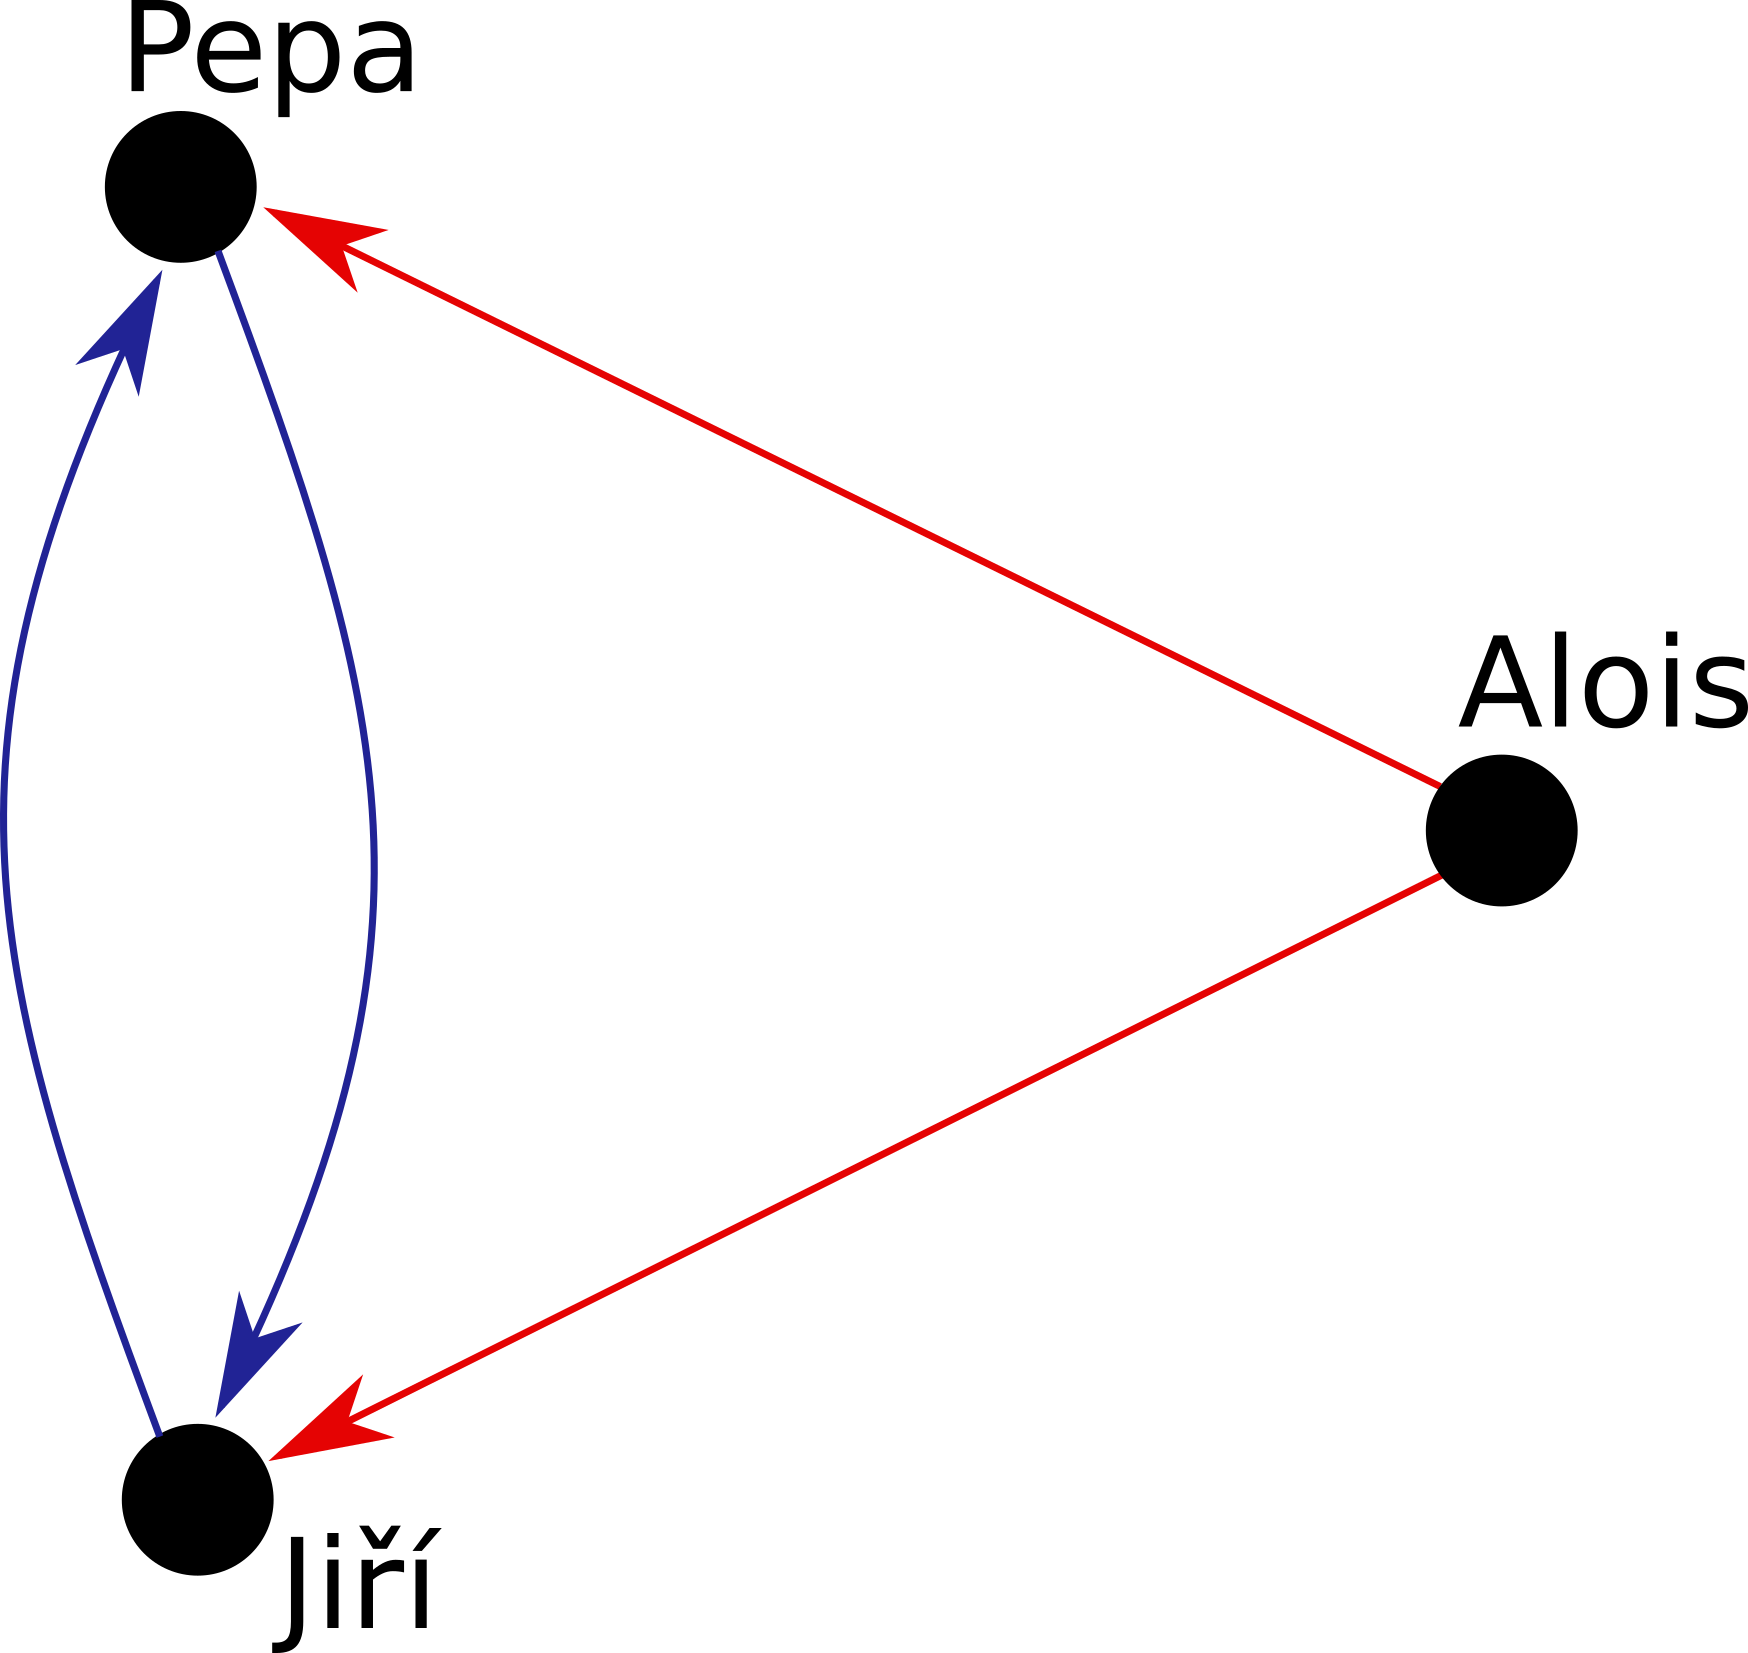
\includegraphics[scale=0.35]{./Pics/pepa.png}
    \end{columns}
\end{frame}
% ############################################
% ############################################
\begin{frame}{Methodology}
    \begin{enumerate}
        \begin{large}
        \onslide<1>\item data collection
        \vspace{0.25cm}
        \onslide<1>\item\bfseries studied groups selection
        \vspace{0.25cm}
        \onslide<0>\item content affecting studied people
        \vspace{0.25cm}
        \onslide<0>\item posts on given topic
        \vspace{0.25cm}
        \onslide<0>\item sentimental analysis
        \vspace{0.25cm}
        \onslide<0>\item filter bubble measures
        \end{large}
    \end{enumerate}
\end{frame}
% ############################################
% ############################################
\begin{frame}{Výběr studované skupiny}
    \vspace{-0.7cm}
    \begin{columns}
    \column{5cm}
    	\begin{itemize}
    		\item studied group
    		\item \textbf{coresponding community}
    		\item random sample from followers
    	\end{itemize}
    \column{6cm}
    	\center
    	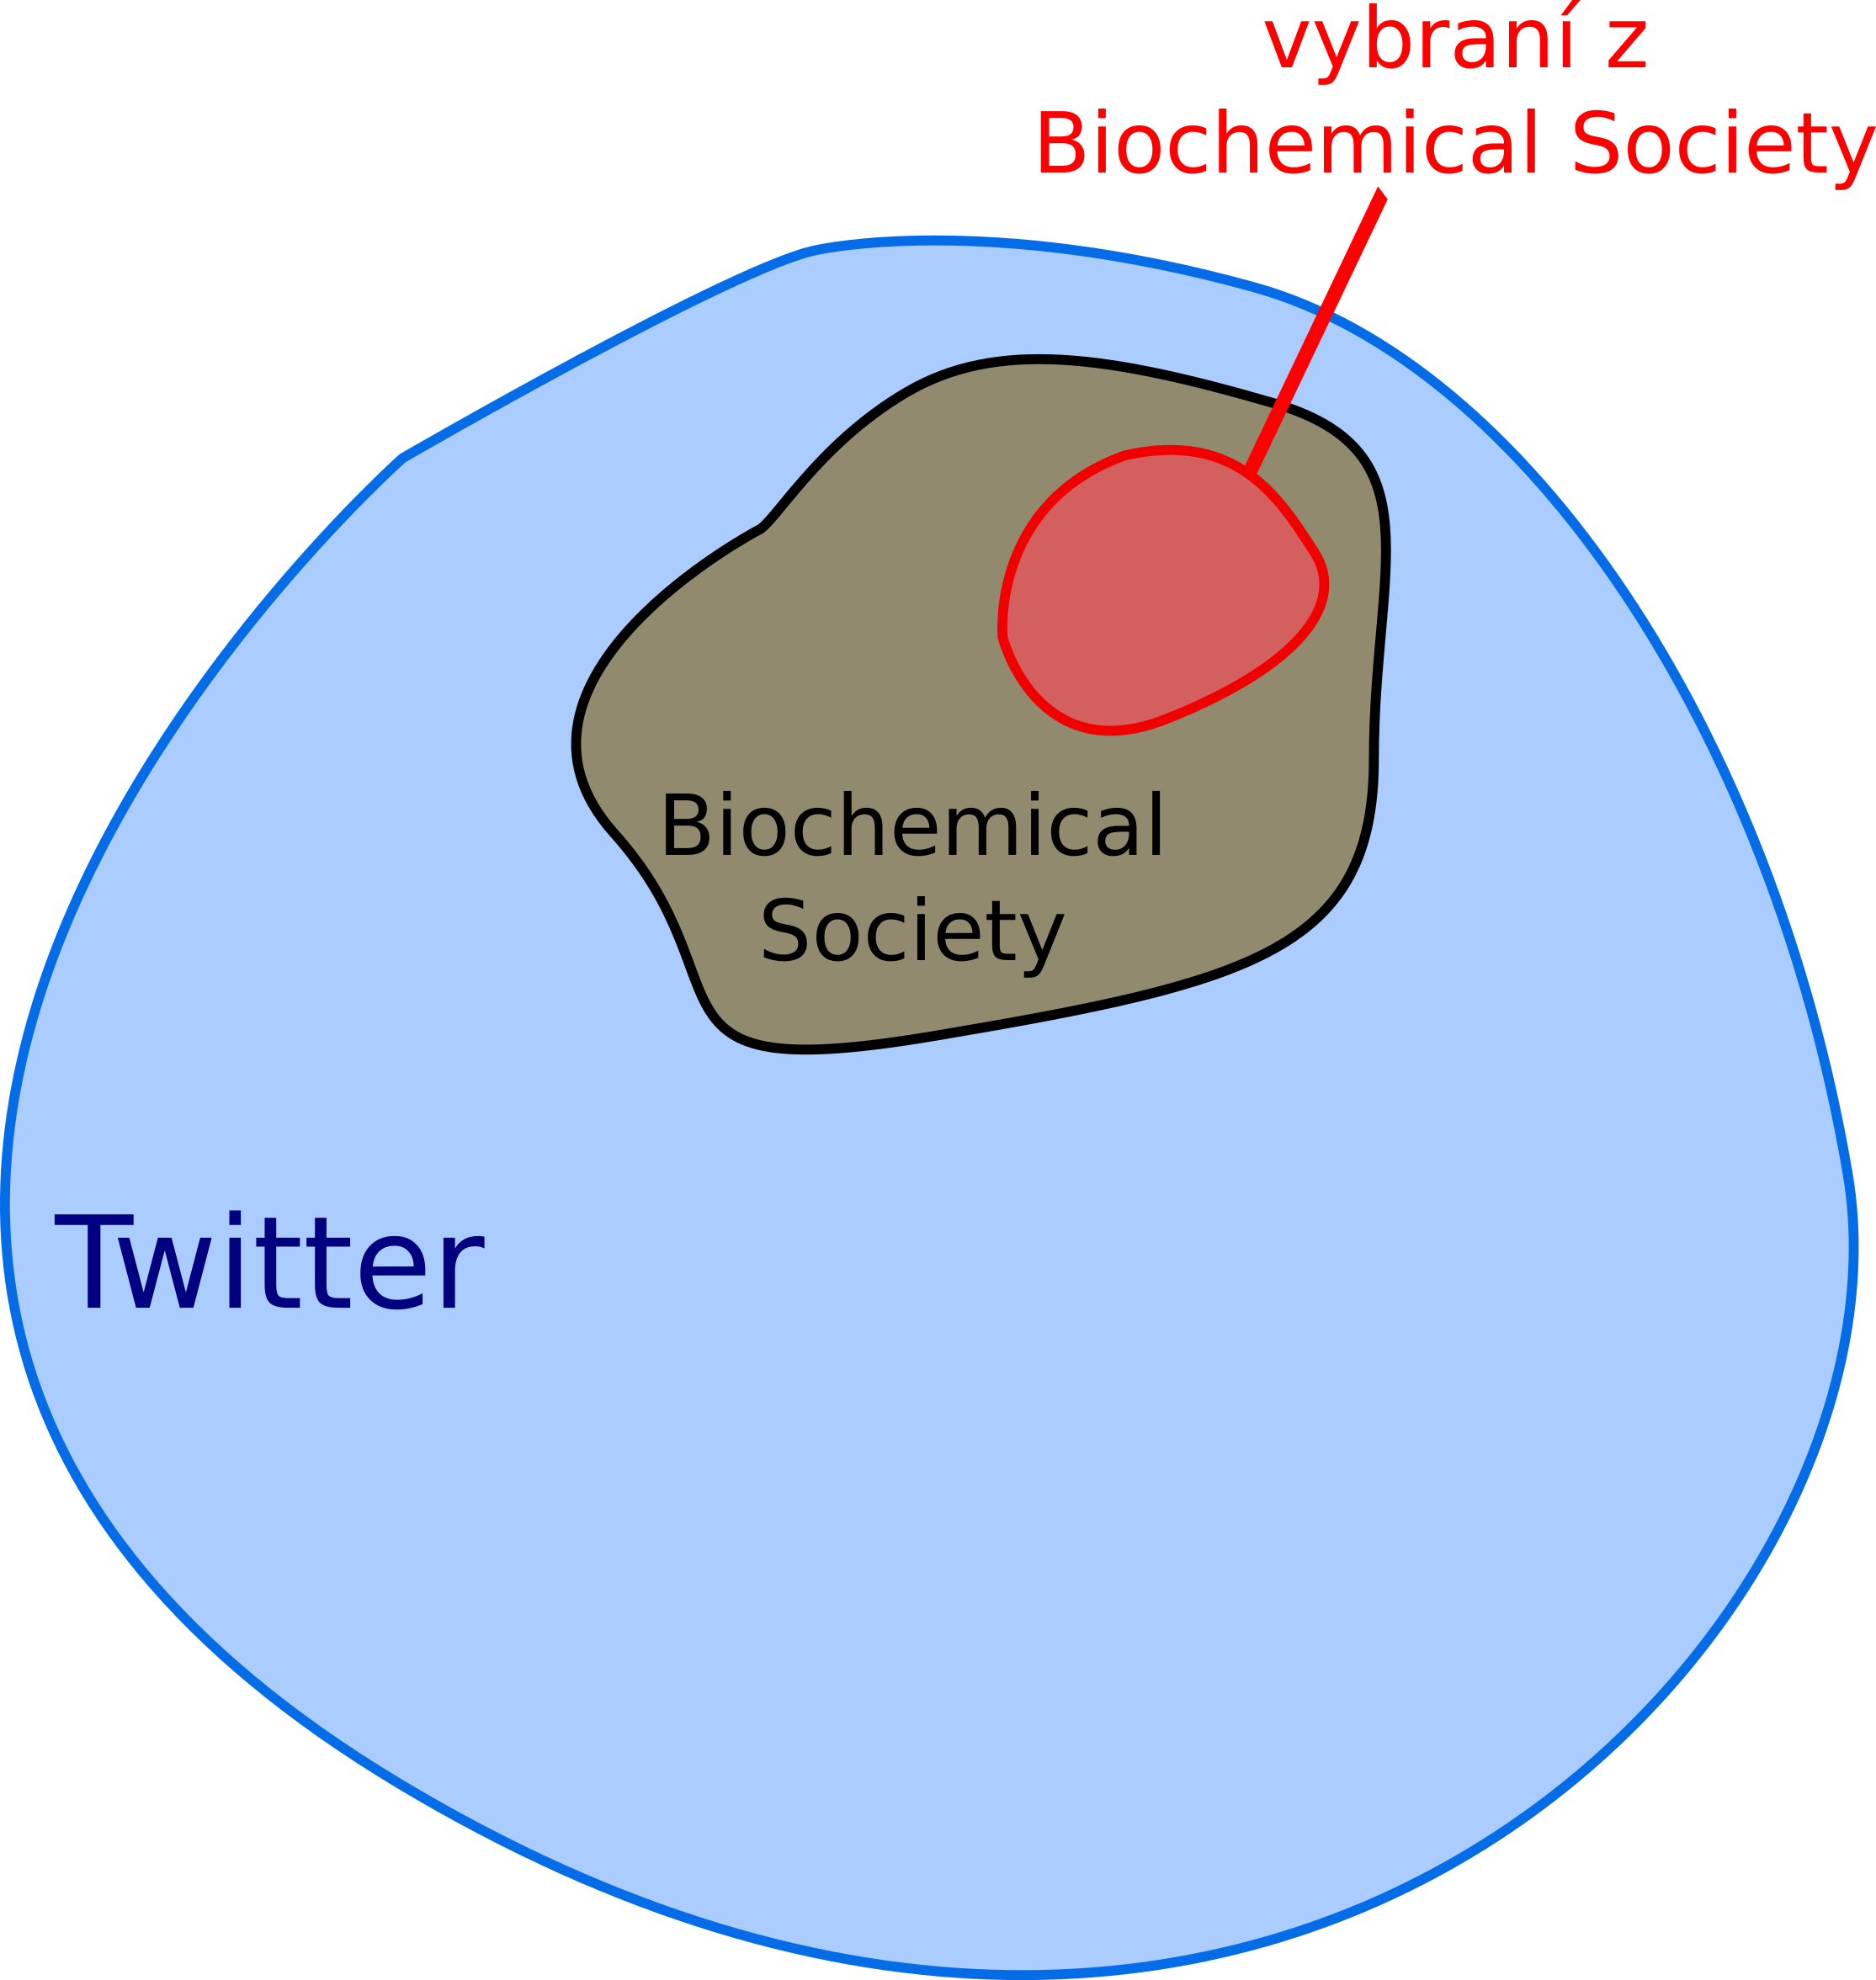
\includegraphics[scale=0.32]{./Pics/sets.png}
    \end{columns}
    \center
    \begin{large}
        $\text{Twitter} \rightarrow \text{Biochemical Society} \rightarrow \text{\textbf{studied people}}$
    \end{large}
\end{frame}
% ############################################
% ############################################
\begin{frame}{Methodology}
    \begin{enumerate}
        \begin{large}
        \onslide<1>\item data collection
        \vspace{0.25cm}
        \onslide<1>\item studied groups selection
        \vspace{0.25cm}
        \onslide<1>\item\bfseries content affecting studied people
        \vspace{0.25cm}
        \onslide<0>\item posts on given topic
        \vspace{0.25cm}
        \onslide<0>\item sentimental analysis
        \vspace{0.25cm}
        \onslide<0>\item filter bubble measures
        \end{large}
    \end{enumerate}
\end{frame}
% ############################################
% ############################################
\begin{frame}{Tweets collection}
    \begin{columns}
    \column{5cm}
    	\begin{itemize}
            \item content affecting studied people
    		\item content from \textbf{followed people}
    		\item muttual twwets
    	\end{itemize}
    \column{6cm}
    	\center
    	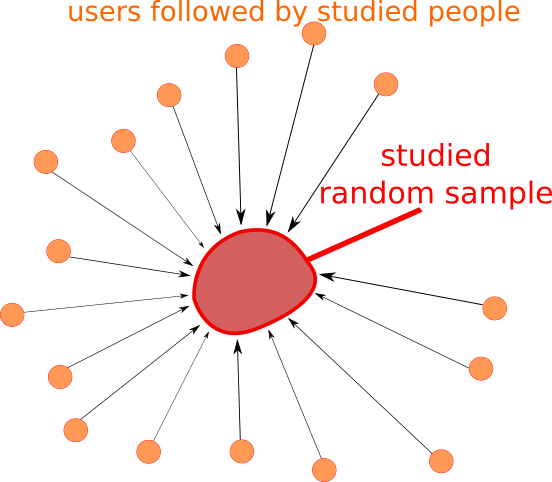
\includegraphics[scale=0.4]{./Pics/followers.png}
    \end{columns}
\end{frame}
% ############################################
% ############################################
\begin{frame}{Methodology}
    \begin{enumerate}
        \begin{large}
        \onslide<1>\item data collection
        \vspace{0.25cm}
        \onslide<1>\item studied groups selection
        \vspace{0.25cm}
        \onslide<1>\item content affecting studied people
        \vspace{0.25cm}
        \onslide<1>\item\bfseries posts on given topic
        \vspace{0.25cm}
        \onslide<0>\item sentimental analysis
        \vspace{0.25cm}
        \onslide<0>\item filter bubble measures
        \end{large}
    \end{enumerate}
\end{frame}
% ############################################
% ############################################
\begin{frame}{Filtrace příspěvků}
\begin{itemize}
    \item posts with given keywords
    \item keyword: \textit{Trump}
\end{itemize}
% \vspace{0.7cm}
\center
I had fish and chips for lunch. \xmark\\
\vspace{0.2cm}
I'm glad Donald \textbf{Trump} is the president of the USA. \cmark\\
\vspace{0.2cm}
The president of the USA is a gentleman. \xmark\\
\end{frame}
% ############################################
% ############################################
\begin{frame}{Methodology}
    \begin{enumerate}
        \begin{large}
        \onslide<1>\item data collection
        \vspace{0.25cm}
        \onslide<1>\item studied groups selection
        \vspace{0.25cm}
        \onslide<1>\item content affecting studied people
        \vspace{0.25cm}
        \onslide<1>\item posts on given topic
        \vspace{0.25cm}
        \onslide<1>\item\bfseries sentimental analysis
        \vspace{0.25cm}
        \onslide<0>\item filter bubble measures
        \end{large}
    \end{enumerate}
\end{frame}
% ############################################
% ############################################
\begin{frame}{Sentimental analysis}
\begin{itemize}
    \item \textbf{positive} vs. \textbf{negative} tweets
    \item classification
    \item machine learning, big data
\end{itemize}
% \vspace{0.7cm}
\center
\textit{Donald Trump is a terrible person.}\\
\textbf{(0.14)}\\
\vspace{0.5cm}
\textit{Donald Trump is a great person.}\\
\textbf{(0.95)}
\end{frame}
% ############################################
% ############################################
\begin{frame}{Methodology}
    \begin{enumerate}
        \begin{large}
        \onslide<1>\item data collection
        \vspace{0.25cm}
        \onslide<1>\item studied groups selection
        \vspace{0.25cm}
        \onslide<1>\item content affecting studied people
        \vspace{0.25cm}
        \onslide<1>\item posts on given topic
        \vspace{0.25cm}
        \onslide<1>\item sentimental analysis
        \vspace{0.25cm}
        \onslide<1>\item\bfseries filter bubble measures
        \end{large}
    \end{enumerate}
\end{frame}
% ############################################
% ############################################
\begin{frame}{Keyword: Trump}
    \vspace{-1cm}
    \begin{figure}
        \centering
        \hspace{-0.5cm}
        \subfloat[]{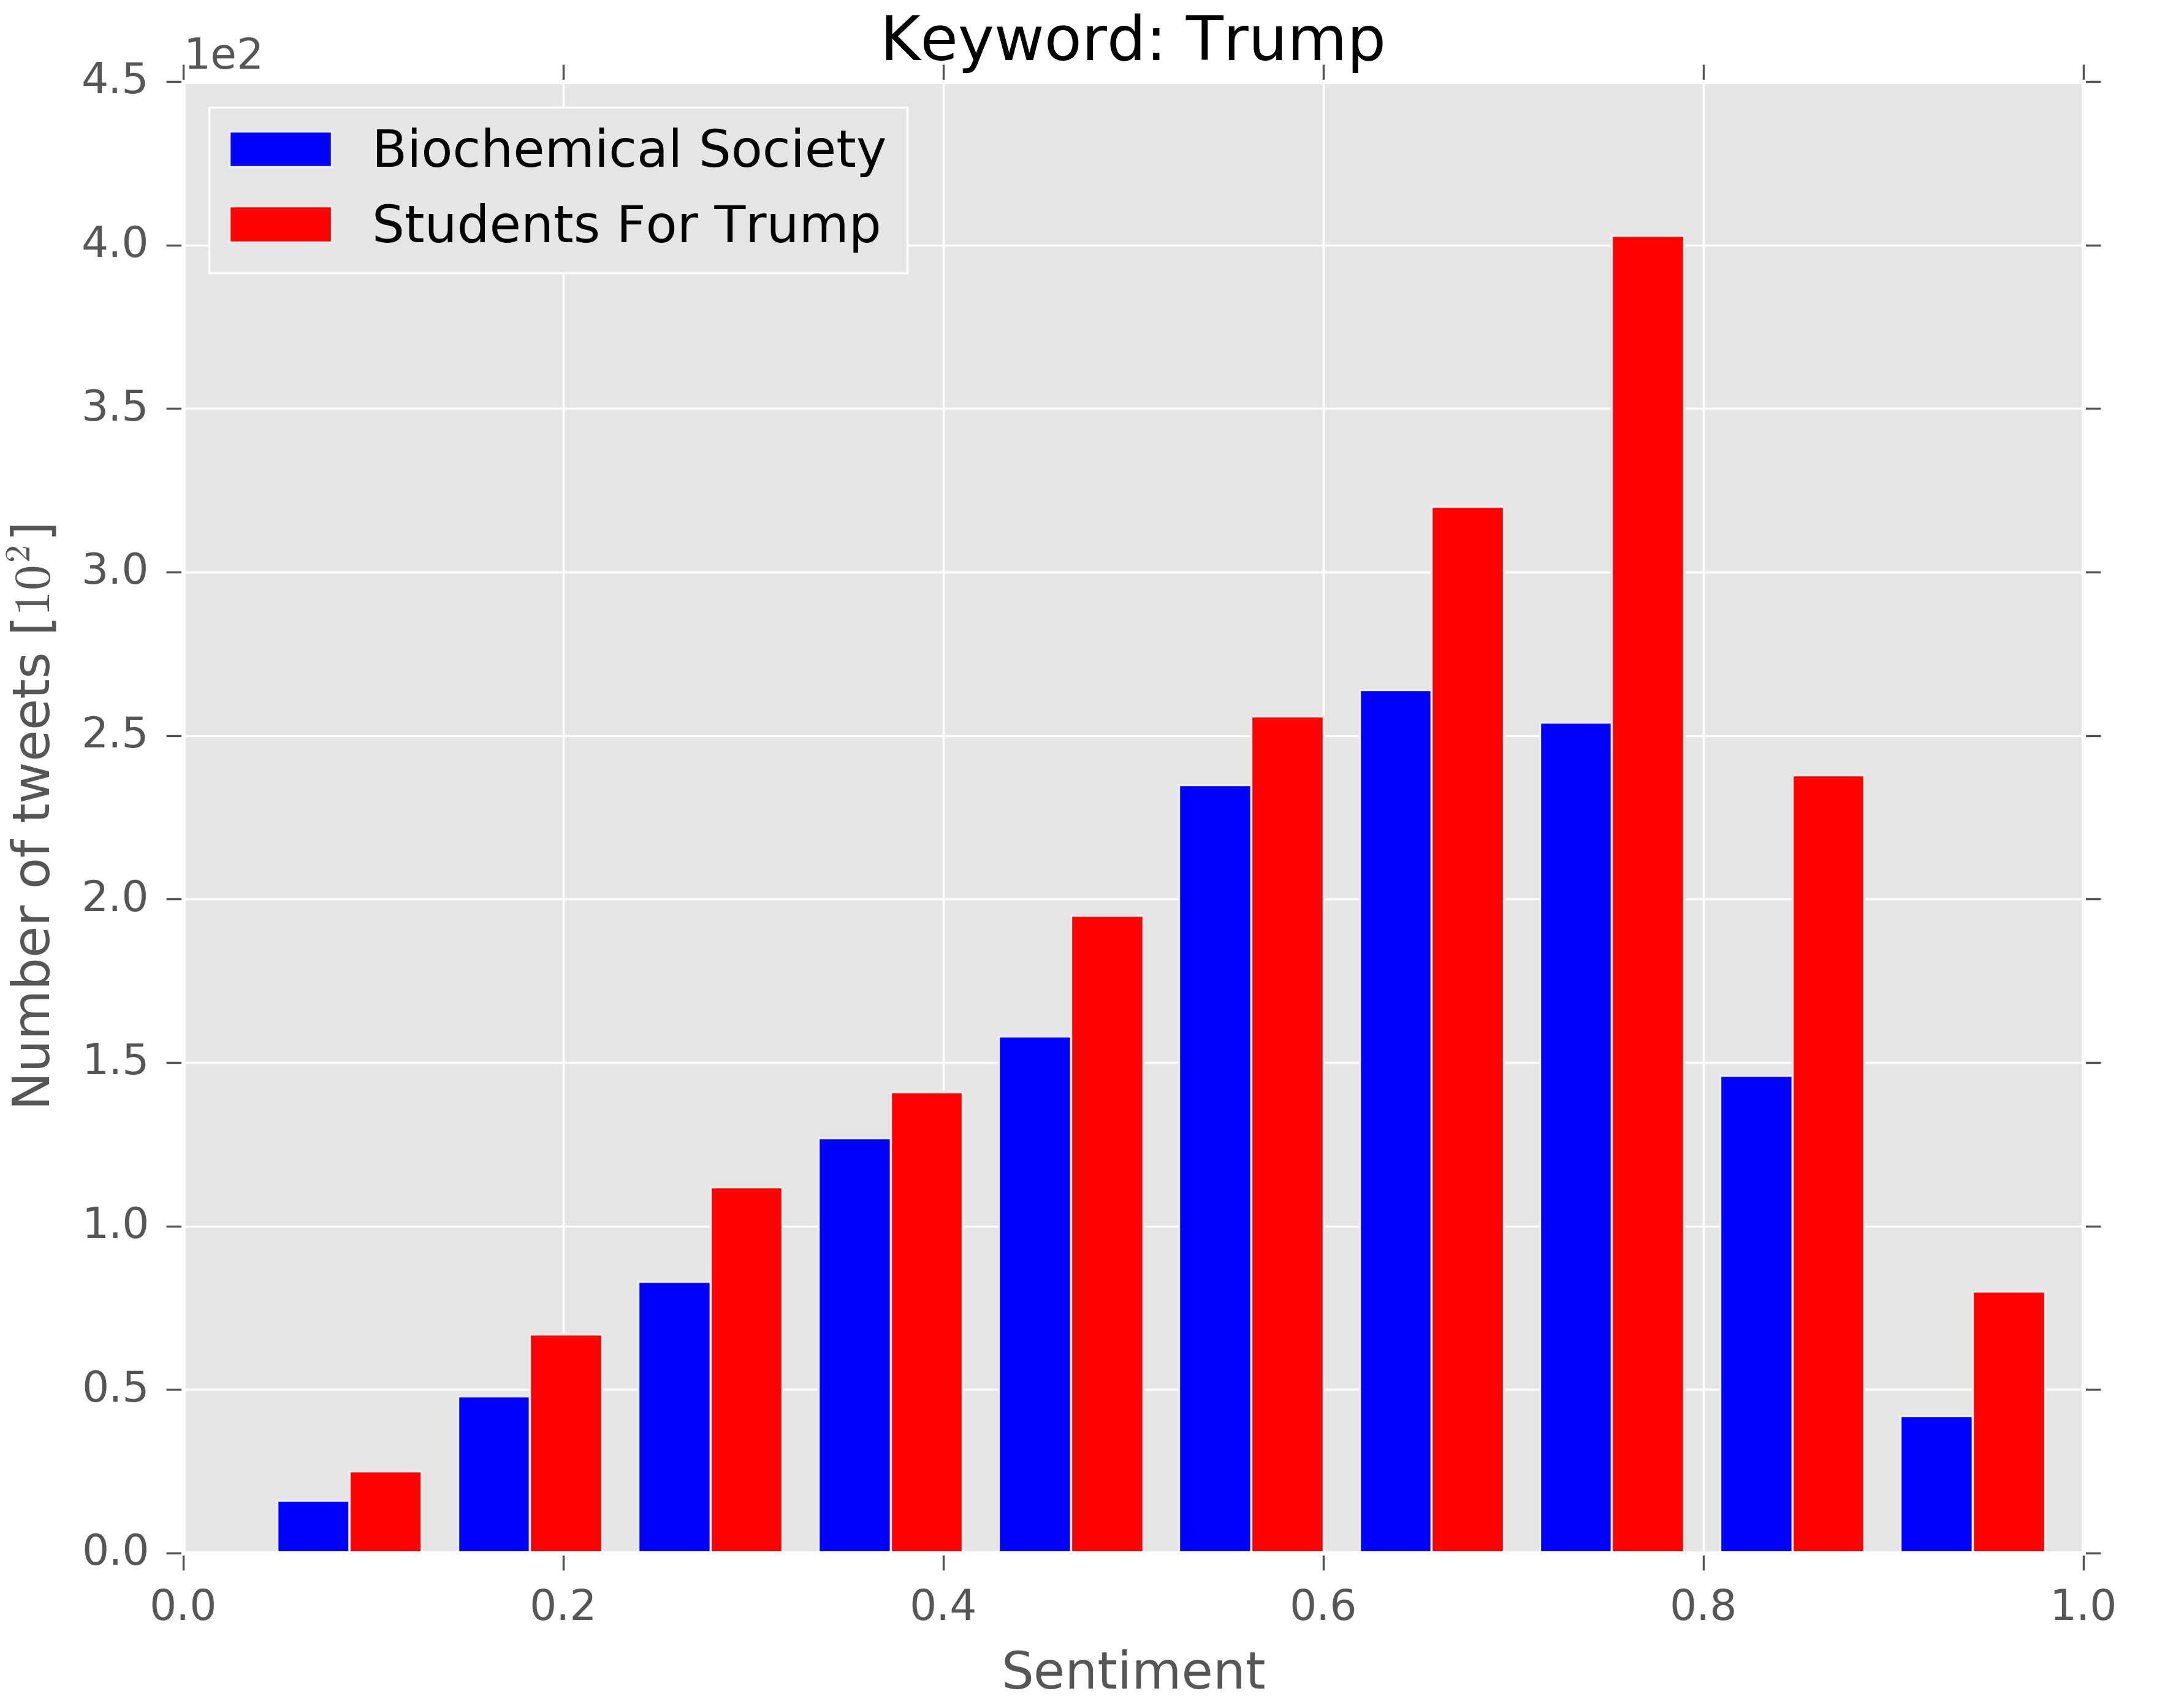
\includegraphics[scale=0.31]{./Pics/trump.png}}
        \subfloat[]{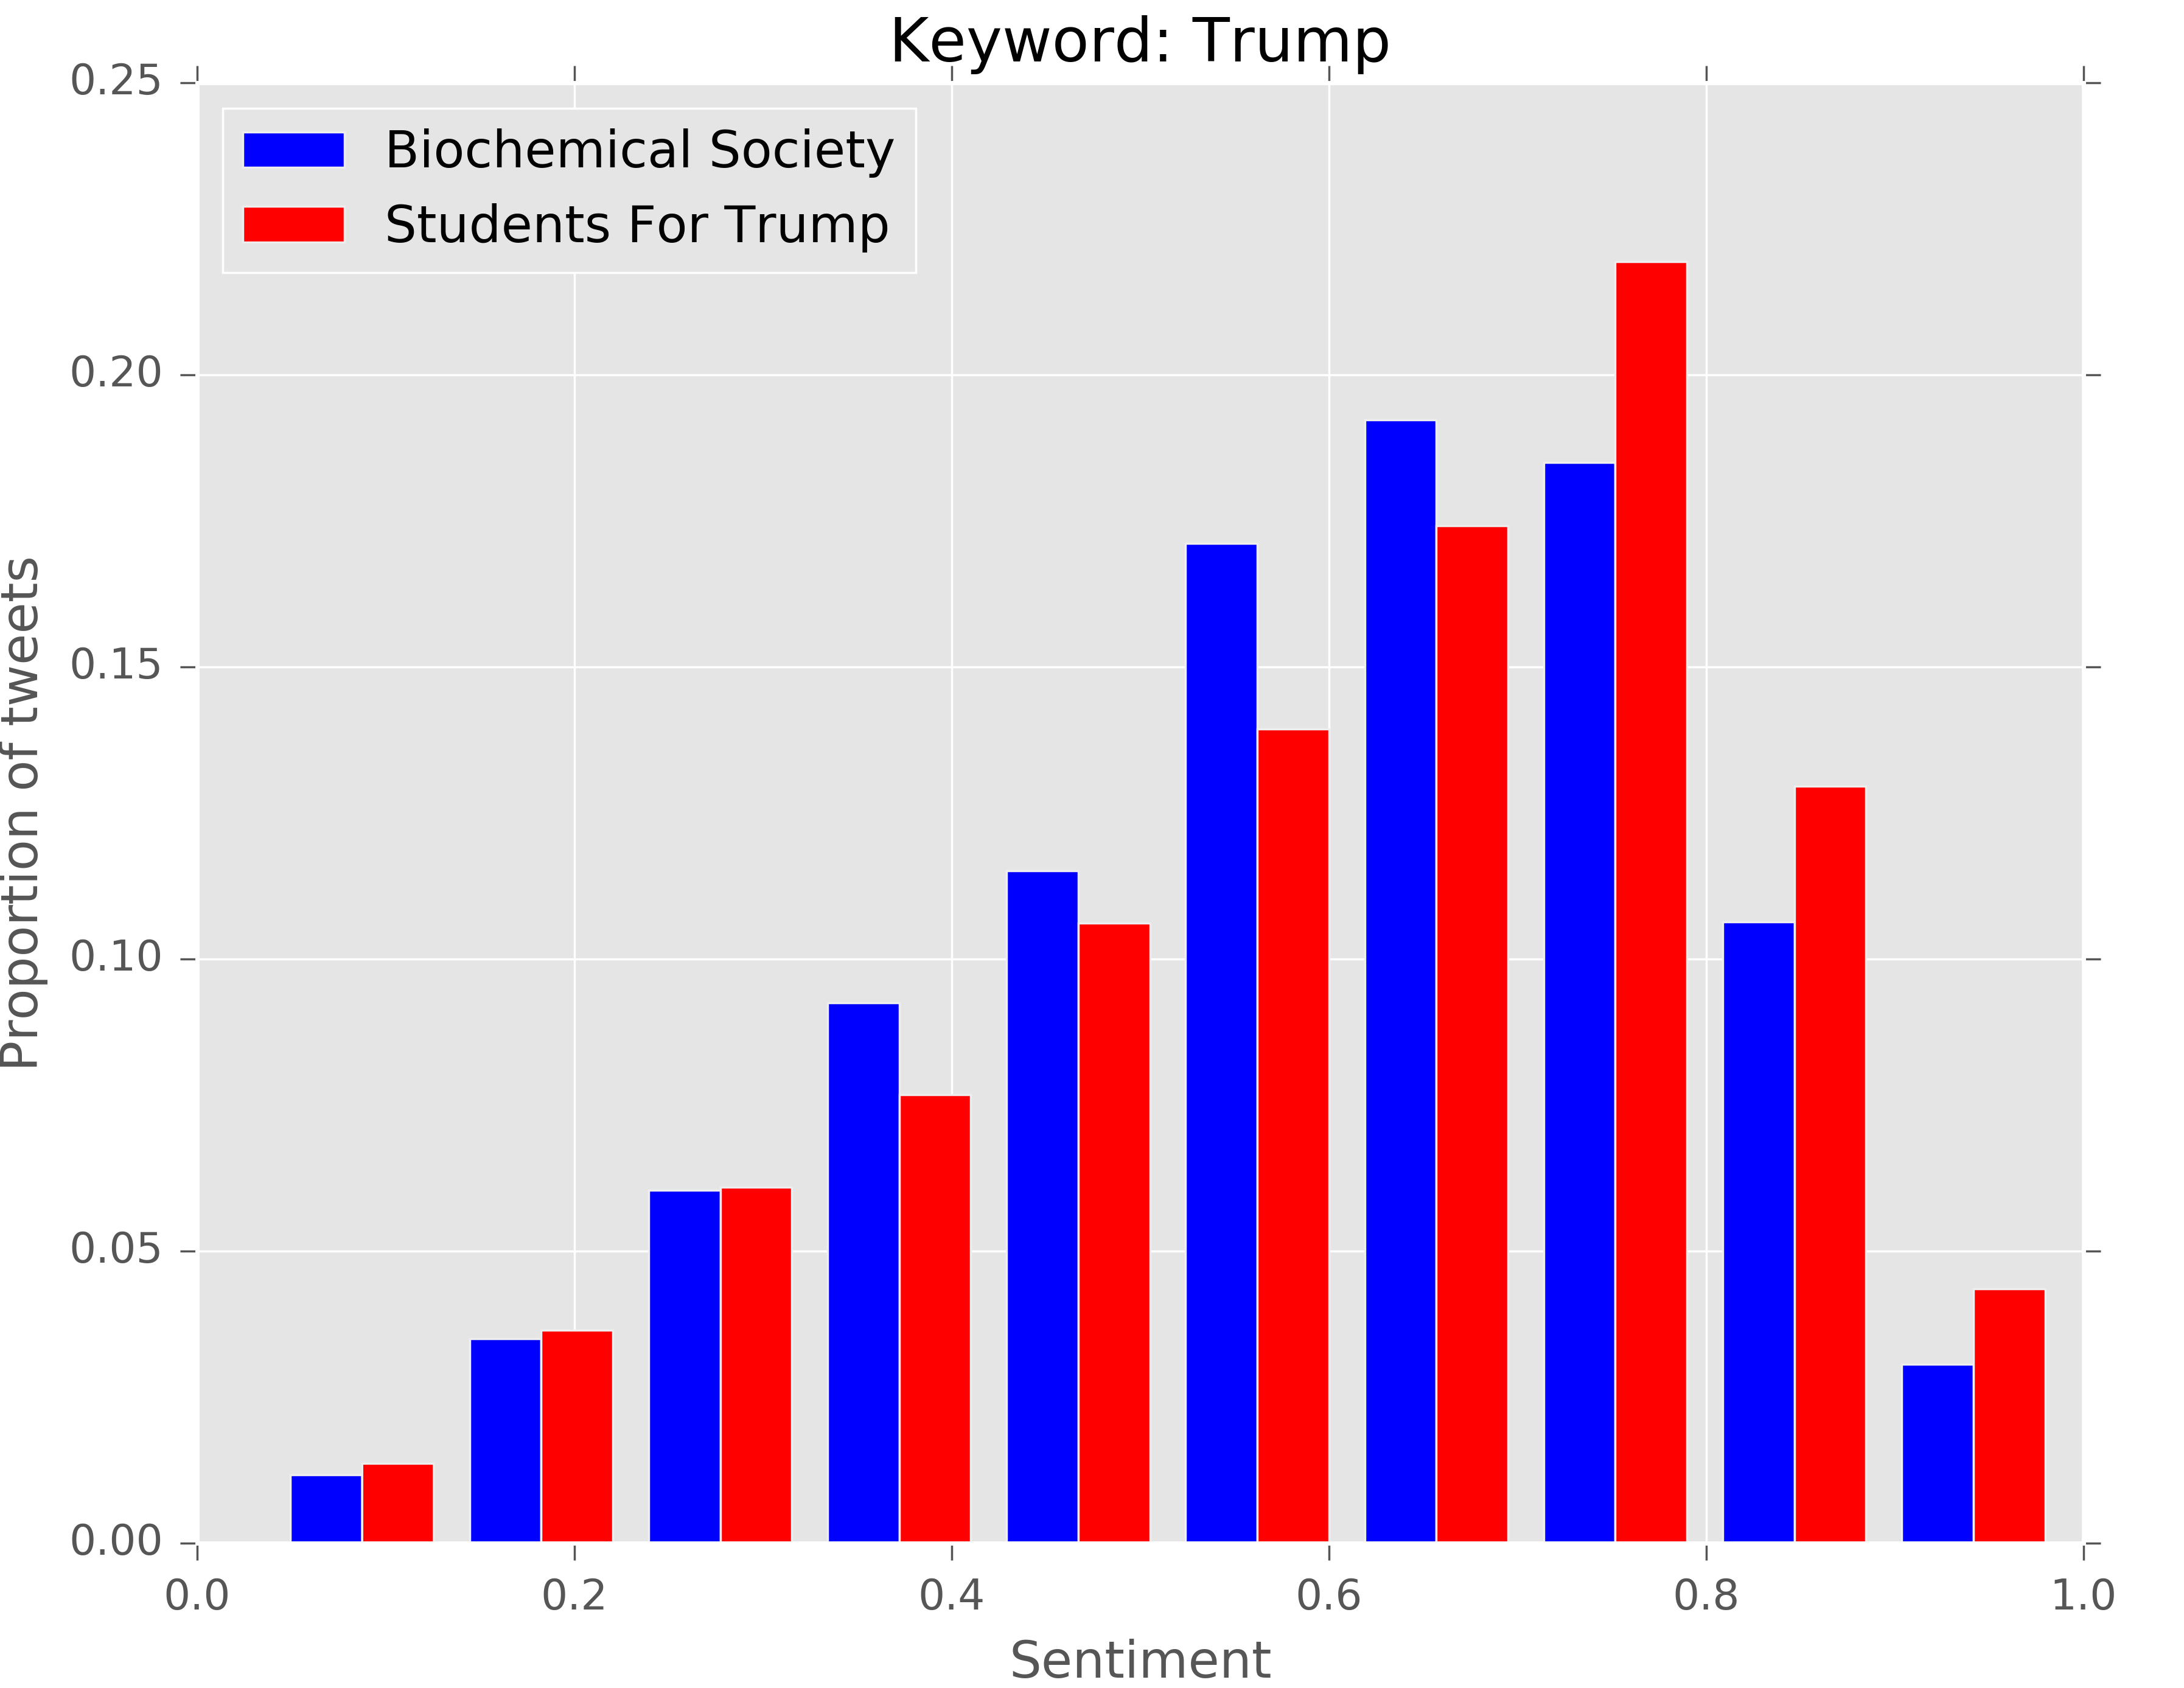
\includegraphics[scale=0.31]{./Pics/trump-normed.png}}
        \vspace{-0.7cm}
        \caption*{Number of tweets histogram, keyword: \textit{"Trump"}.}
    \end{figure}
	\begin{itemize}
		\item \textit{Biochemical Society}
		\item \textit{Students for Trump}
	\end{itemize}
\end{frame}
% ############################################
\begin{frame}{Keyword: Trump}
    \begin{figure}
        \centering
        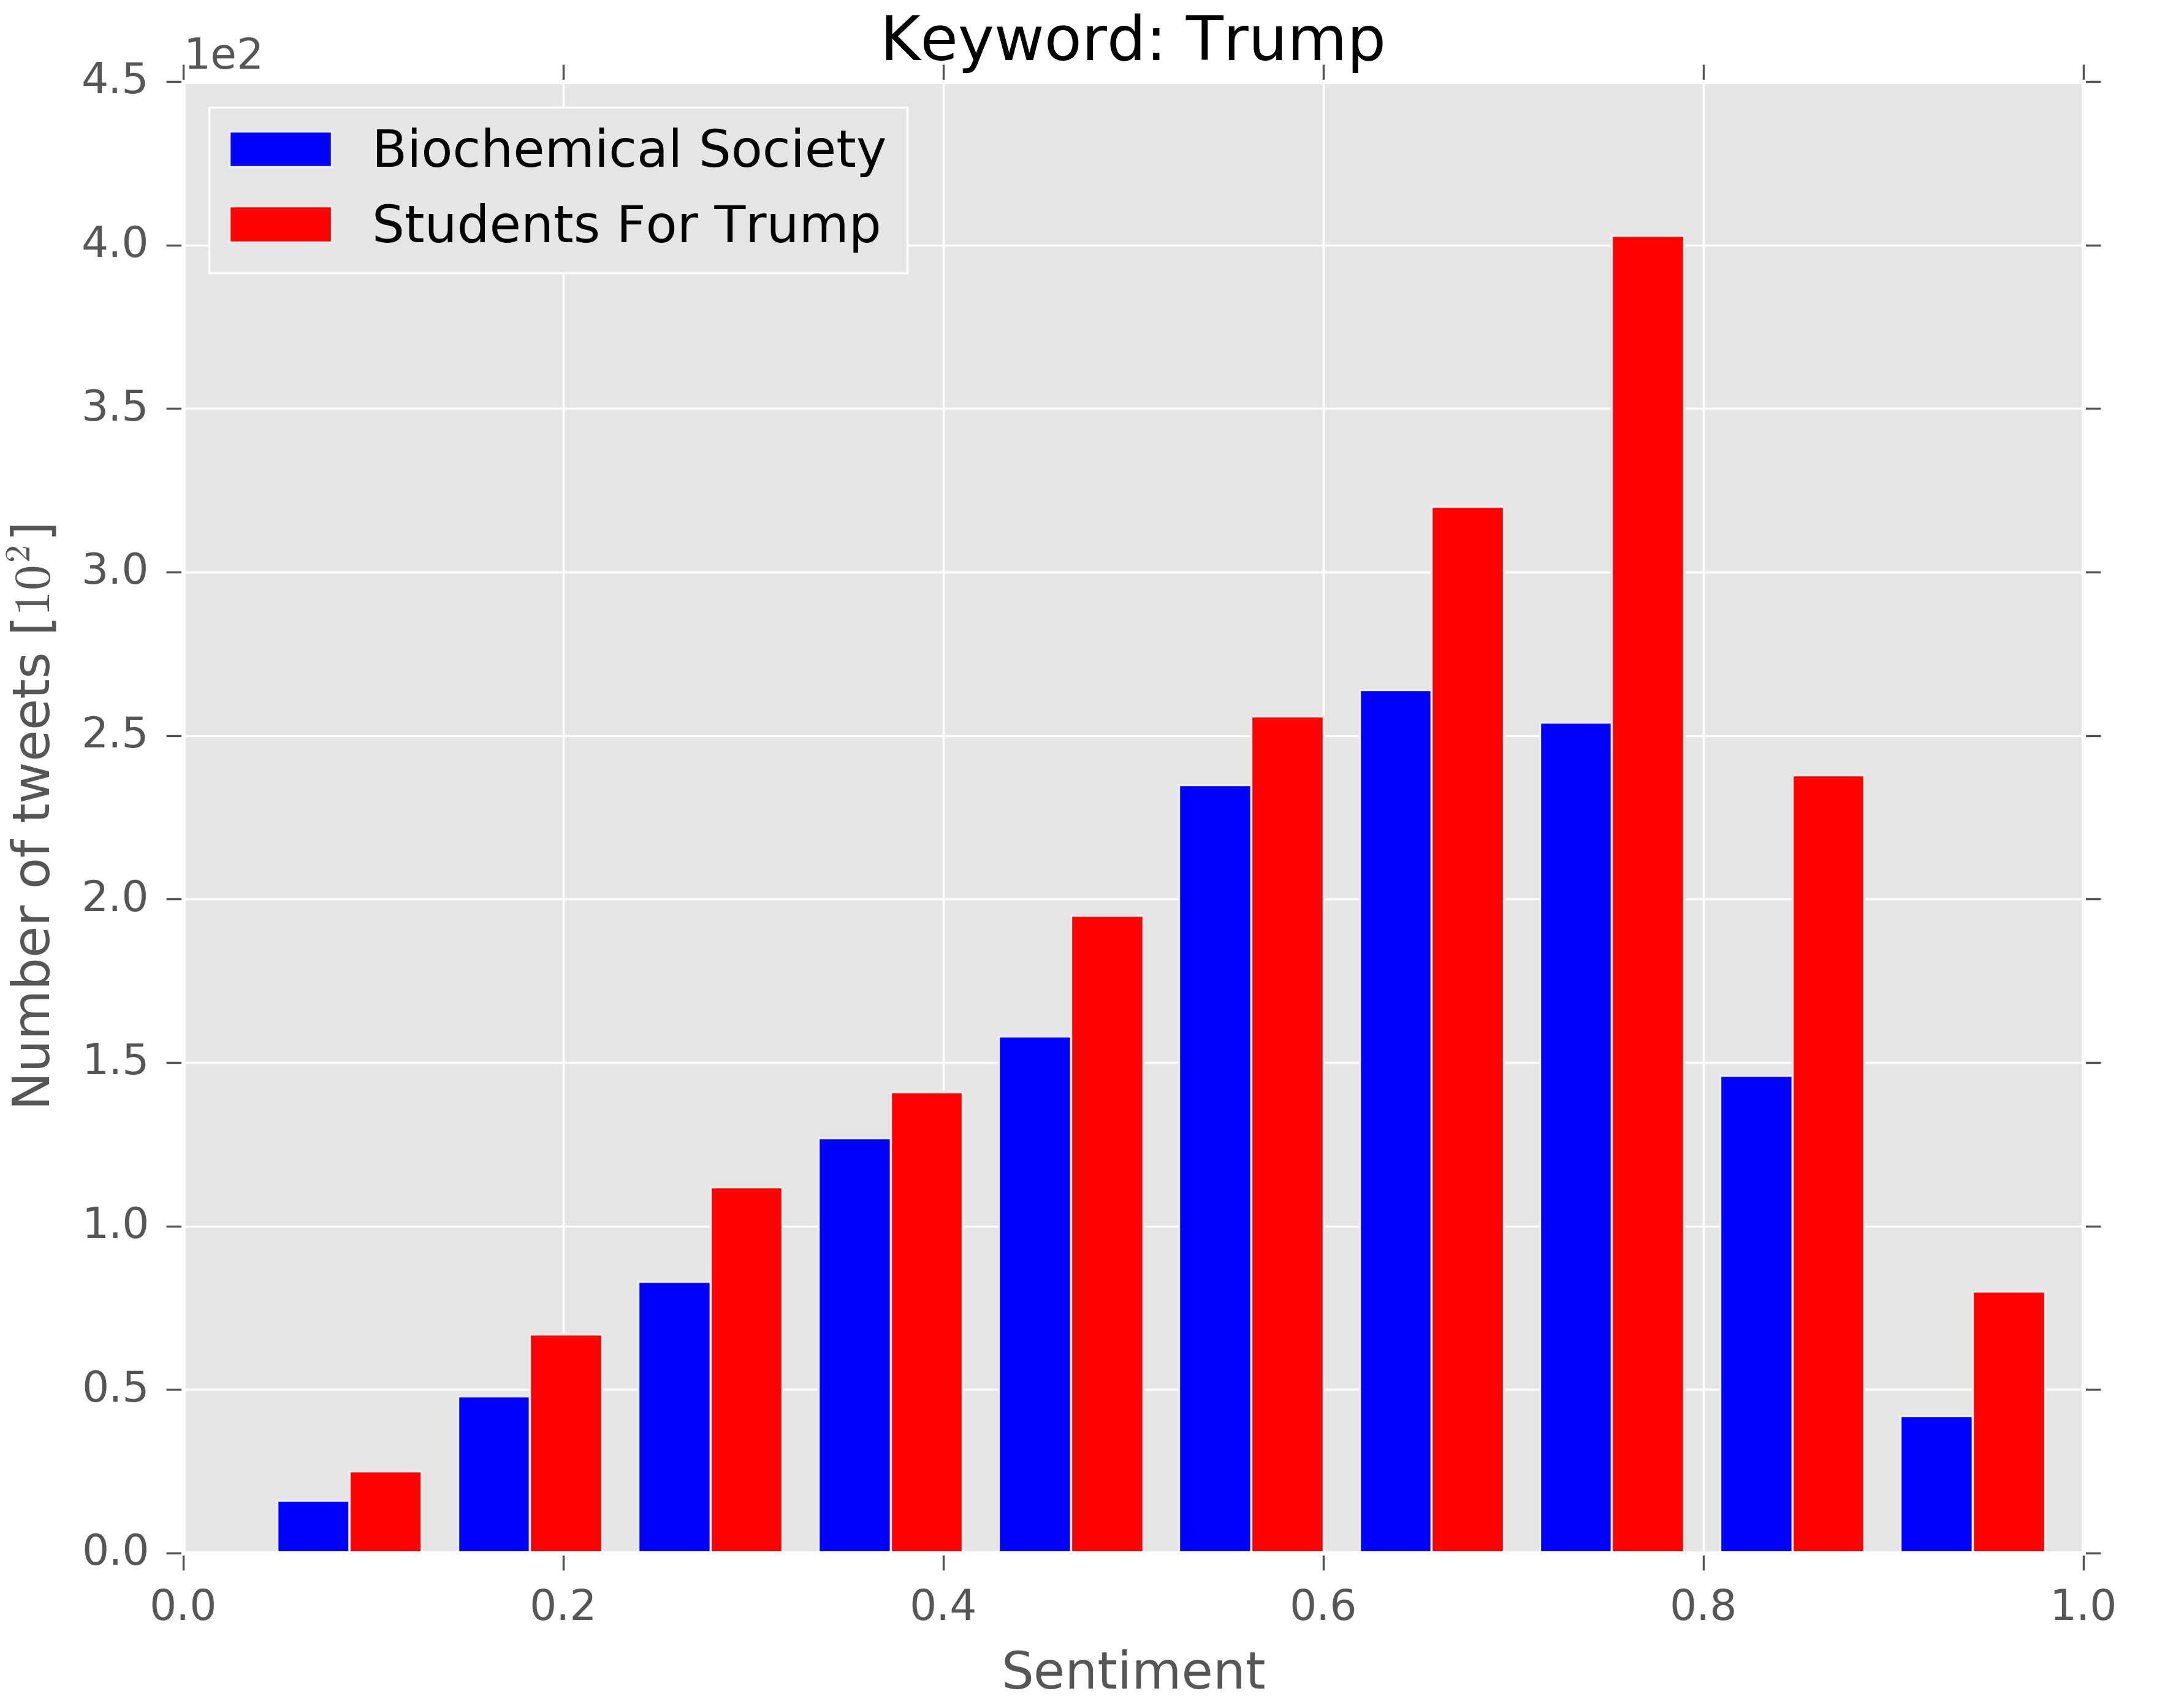
\includegraphics[scale=0.37]{./Pics/trump.png}
    \end{figure}
    \vspace{-0.4cm}
    \begin{itemize}
        \item \textbf{slight difference} in number of tweets
        \item \textit{Students for Trump} slightly more positive
    \end{itemize}
\end{frame}
% ############################################
\begin{frame}{Keyword: Trump}
    \begin{figure}
        \centering
        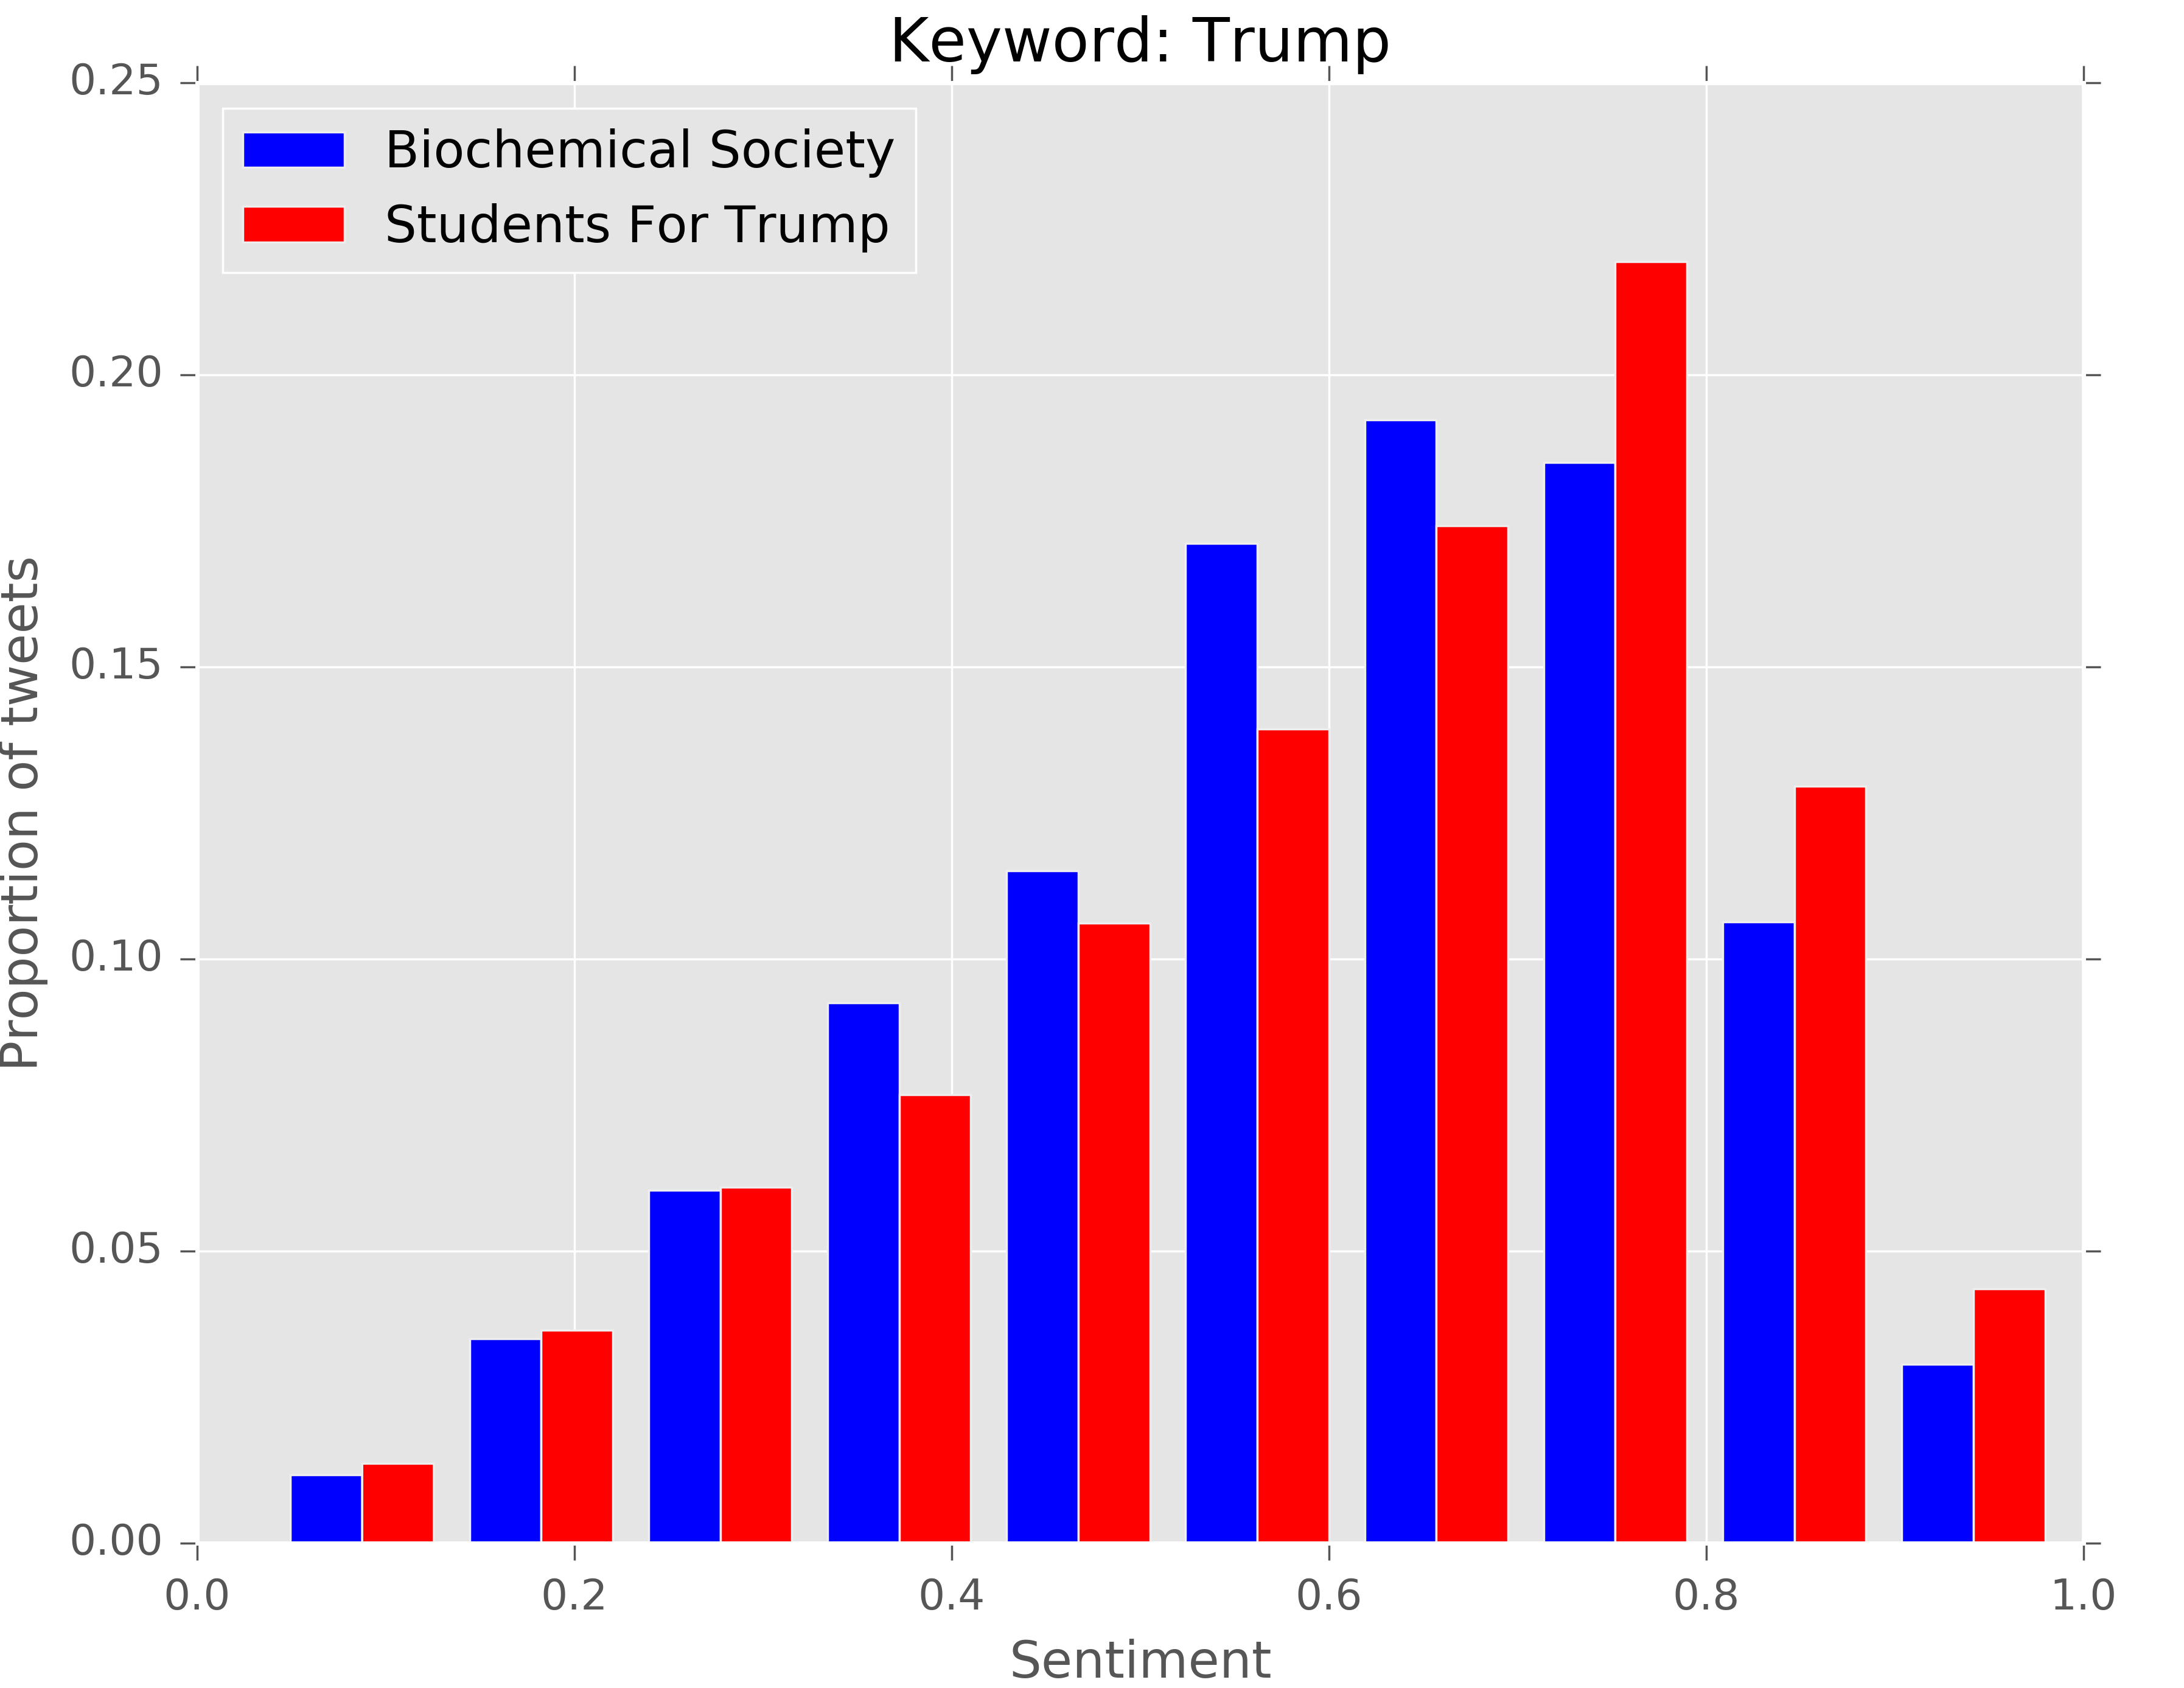
\includegraphics[scale=0.37]{./Pics/trump-normed.png}
        \vspace{-0.2cm}
        \caption*{Normalized histogram - sentiment proportion.}
    \end{figure}
    \vspace{-0.4cm}
	\begin{itemize}
        \item \textit{Biochemical Society} $\rightarrow$ sentiment $< 0.5$
		\item \textit{Students for Trump} $\rightarrow$ sentiment $> 0.5$
	\end{itemize}
\end{frame}
% ############################################
% ############################################
\begin{frame}{Keyword: abortion}
    \vspace{-1cm}
    \begin{figure}
        \centering
        \hspace{-0.5cm}
        \subfloat[]{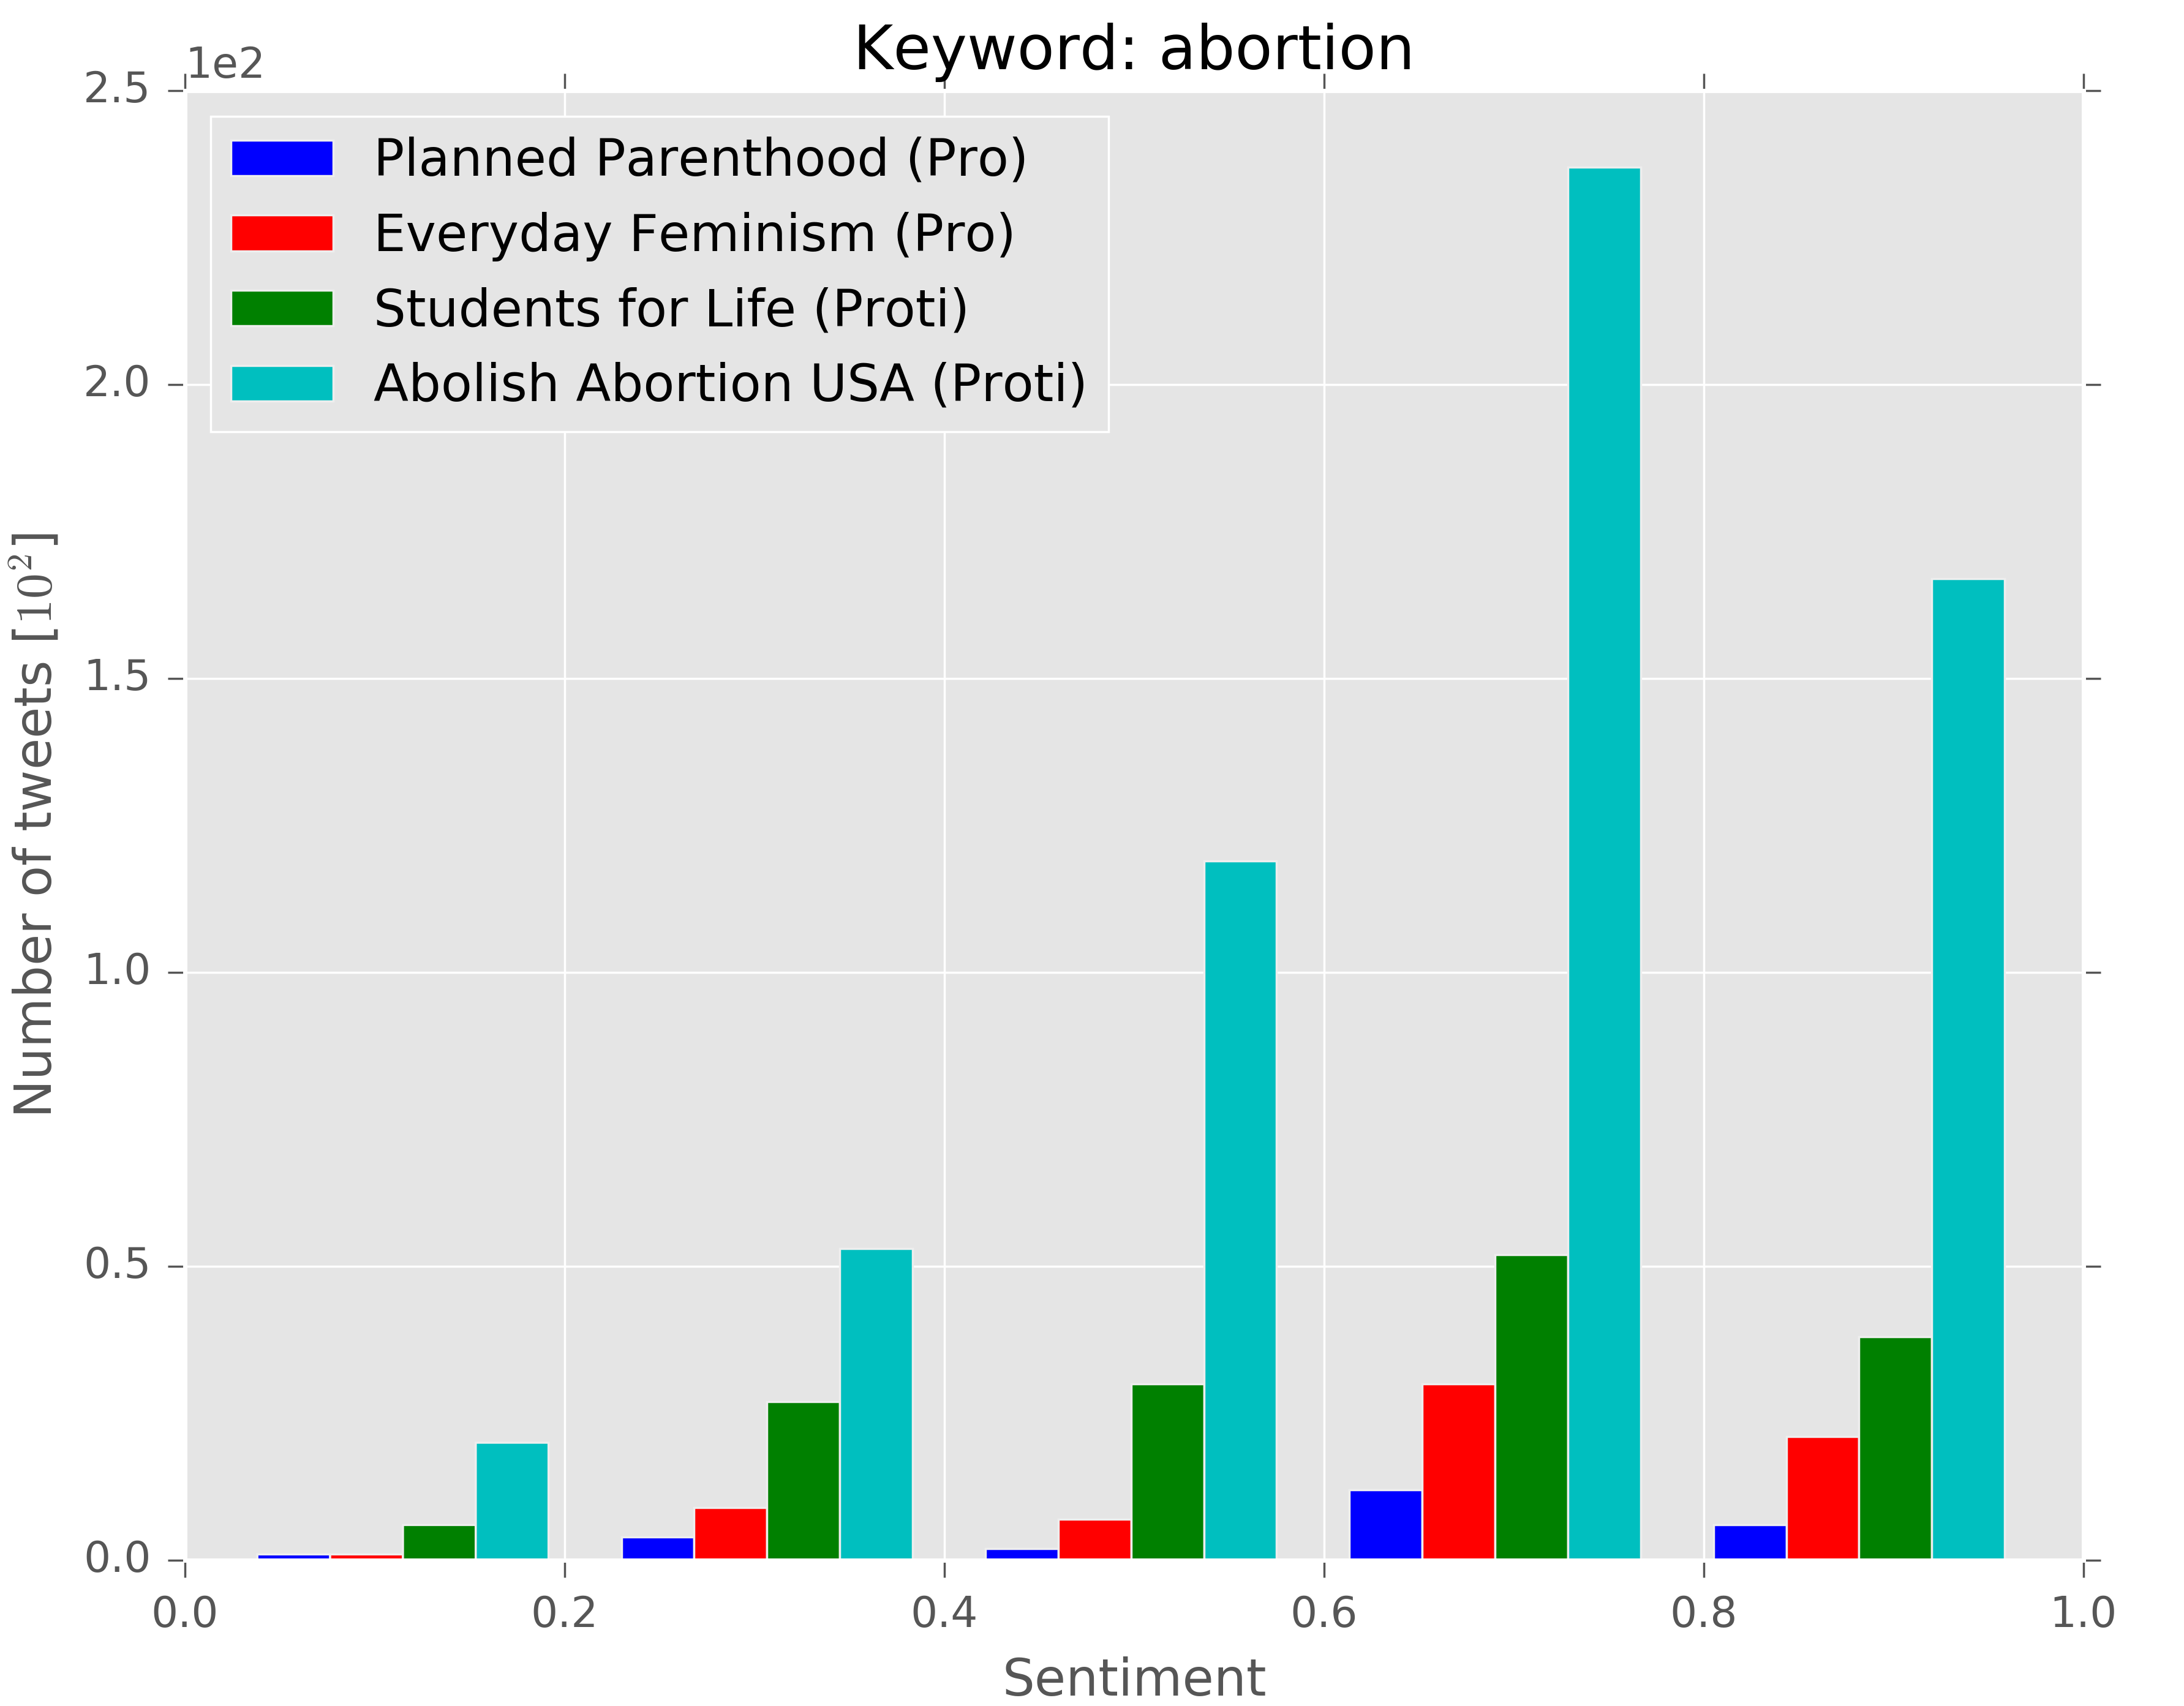
\includegraphics[scale=0.31]{./Pics/abortion.png}}
        \subfloat[]{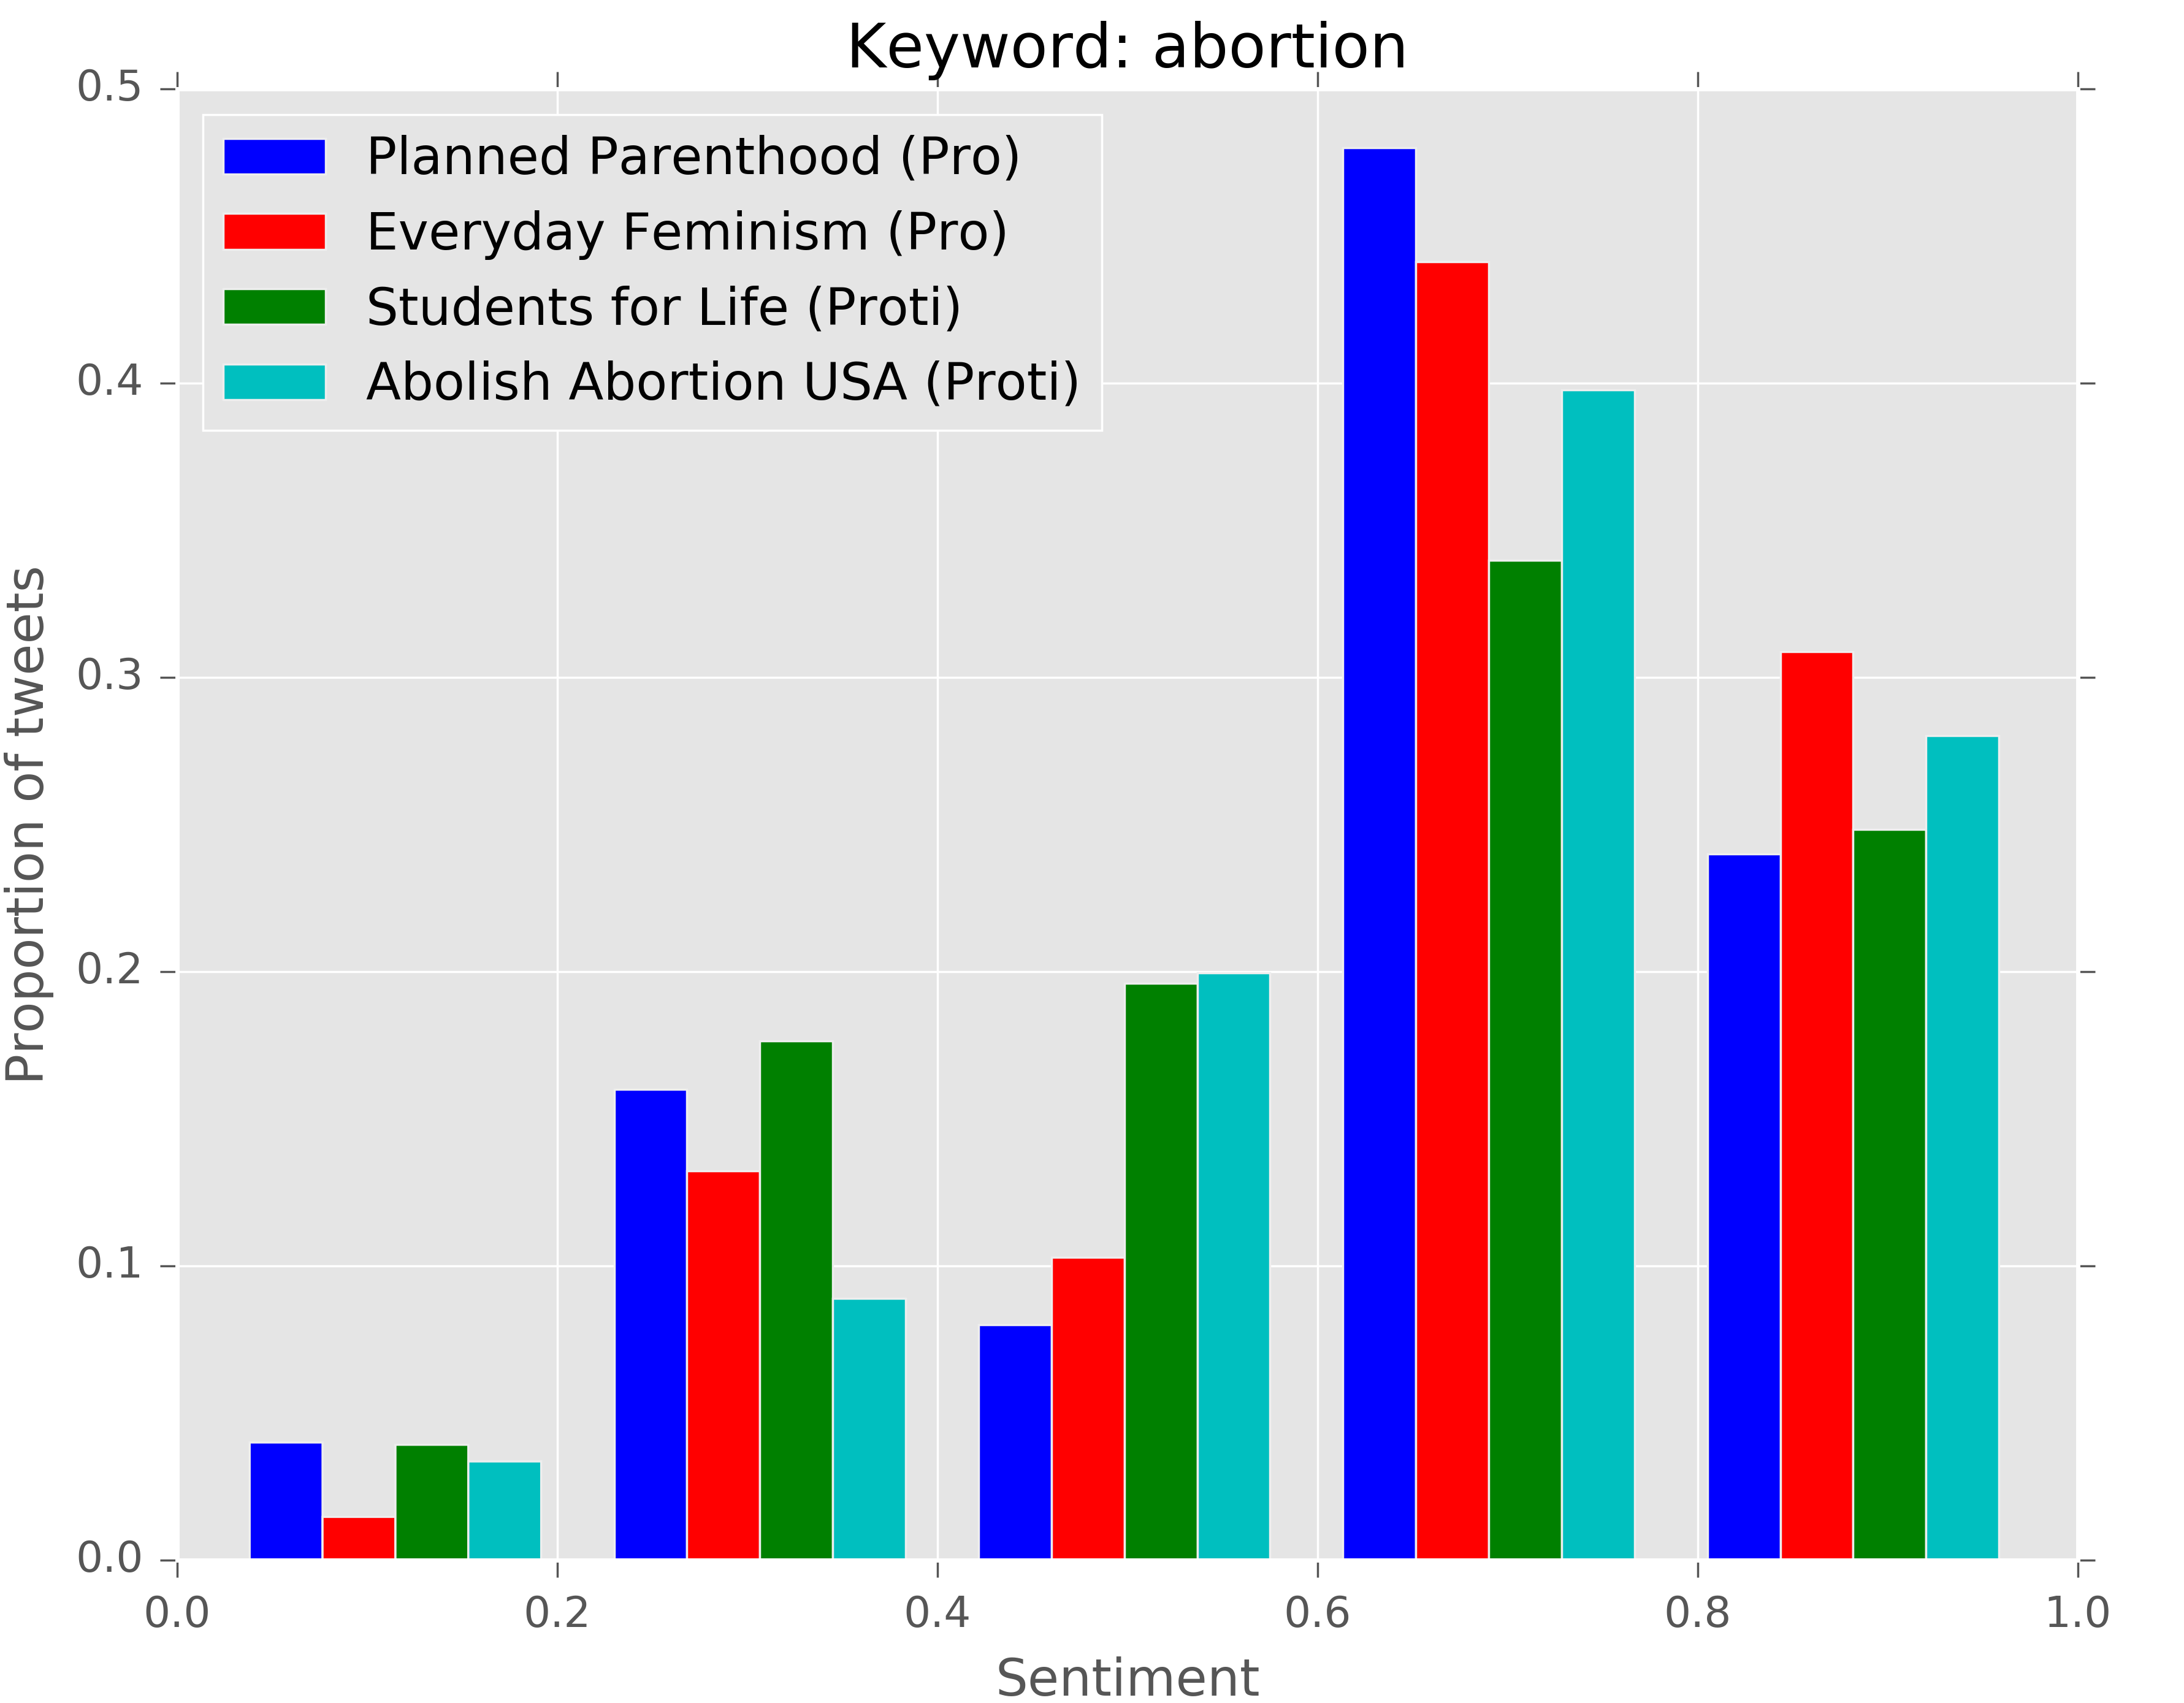
\includegraphics[scale=0.31]{./Pics/abortion-normed.png}}
        \vspace{-0.7cm}
        \caption*{Number of tweets histogram, keyword: \textit{"abortion"}.}
    \end{figure}
    \vspace{-0.3cm}
    \begin{columns}
    \column{6cm}
    	\begin{itemize}
    		\item \textit{Planned Parenthood}
    		\item \textit{Everyday Feminism}
    	\end{itemize}
    \column{6cm}
    	\begin{itemize}
    		\item \textit{Student for Life}
    		\item \textit{Abolish Abortion USA}
    	\end{itemize}
    \end{columns}
\end{frame}
% ############################################
\begin{frame}{Keyword: abortion}
    \begin{figure}
        \centering
        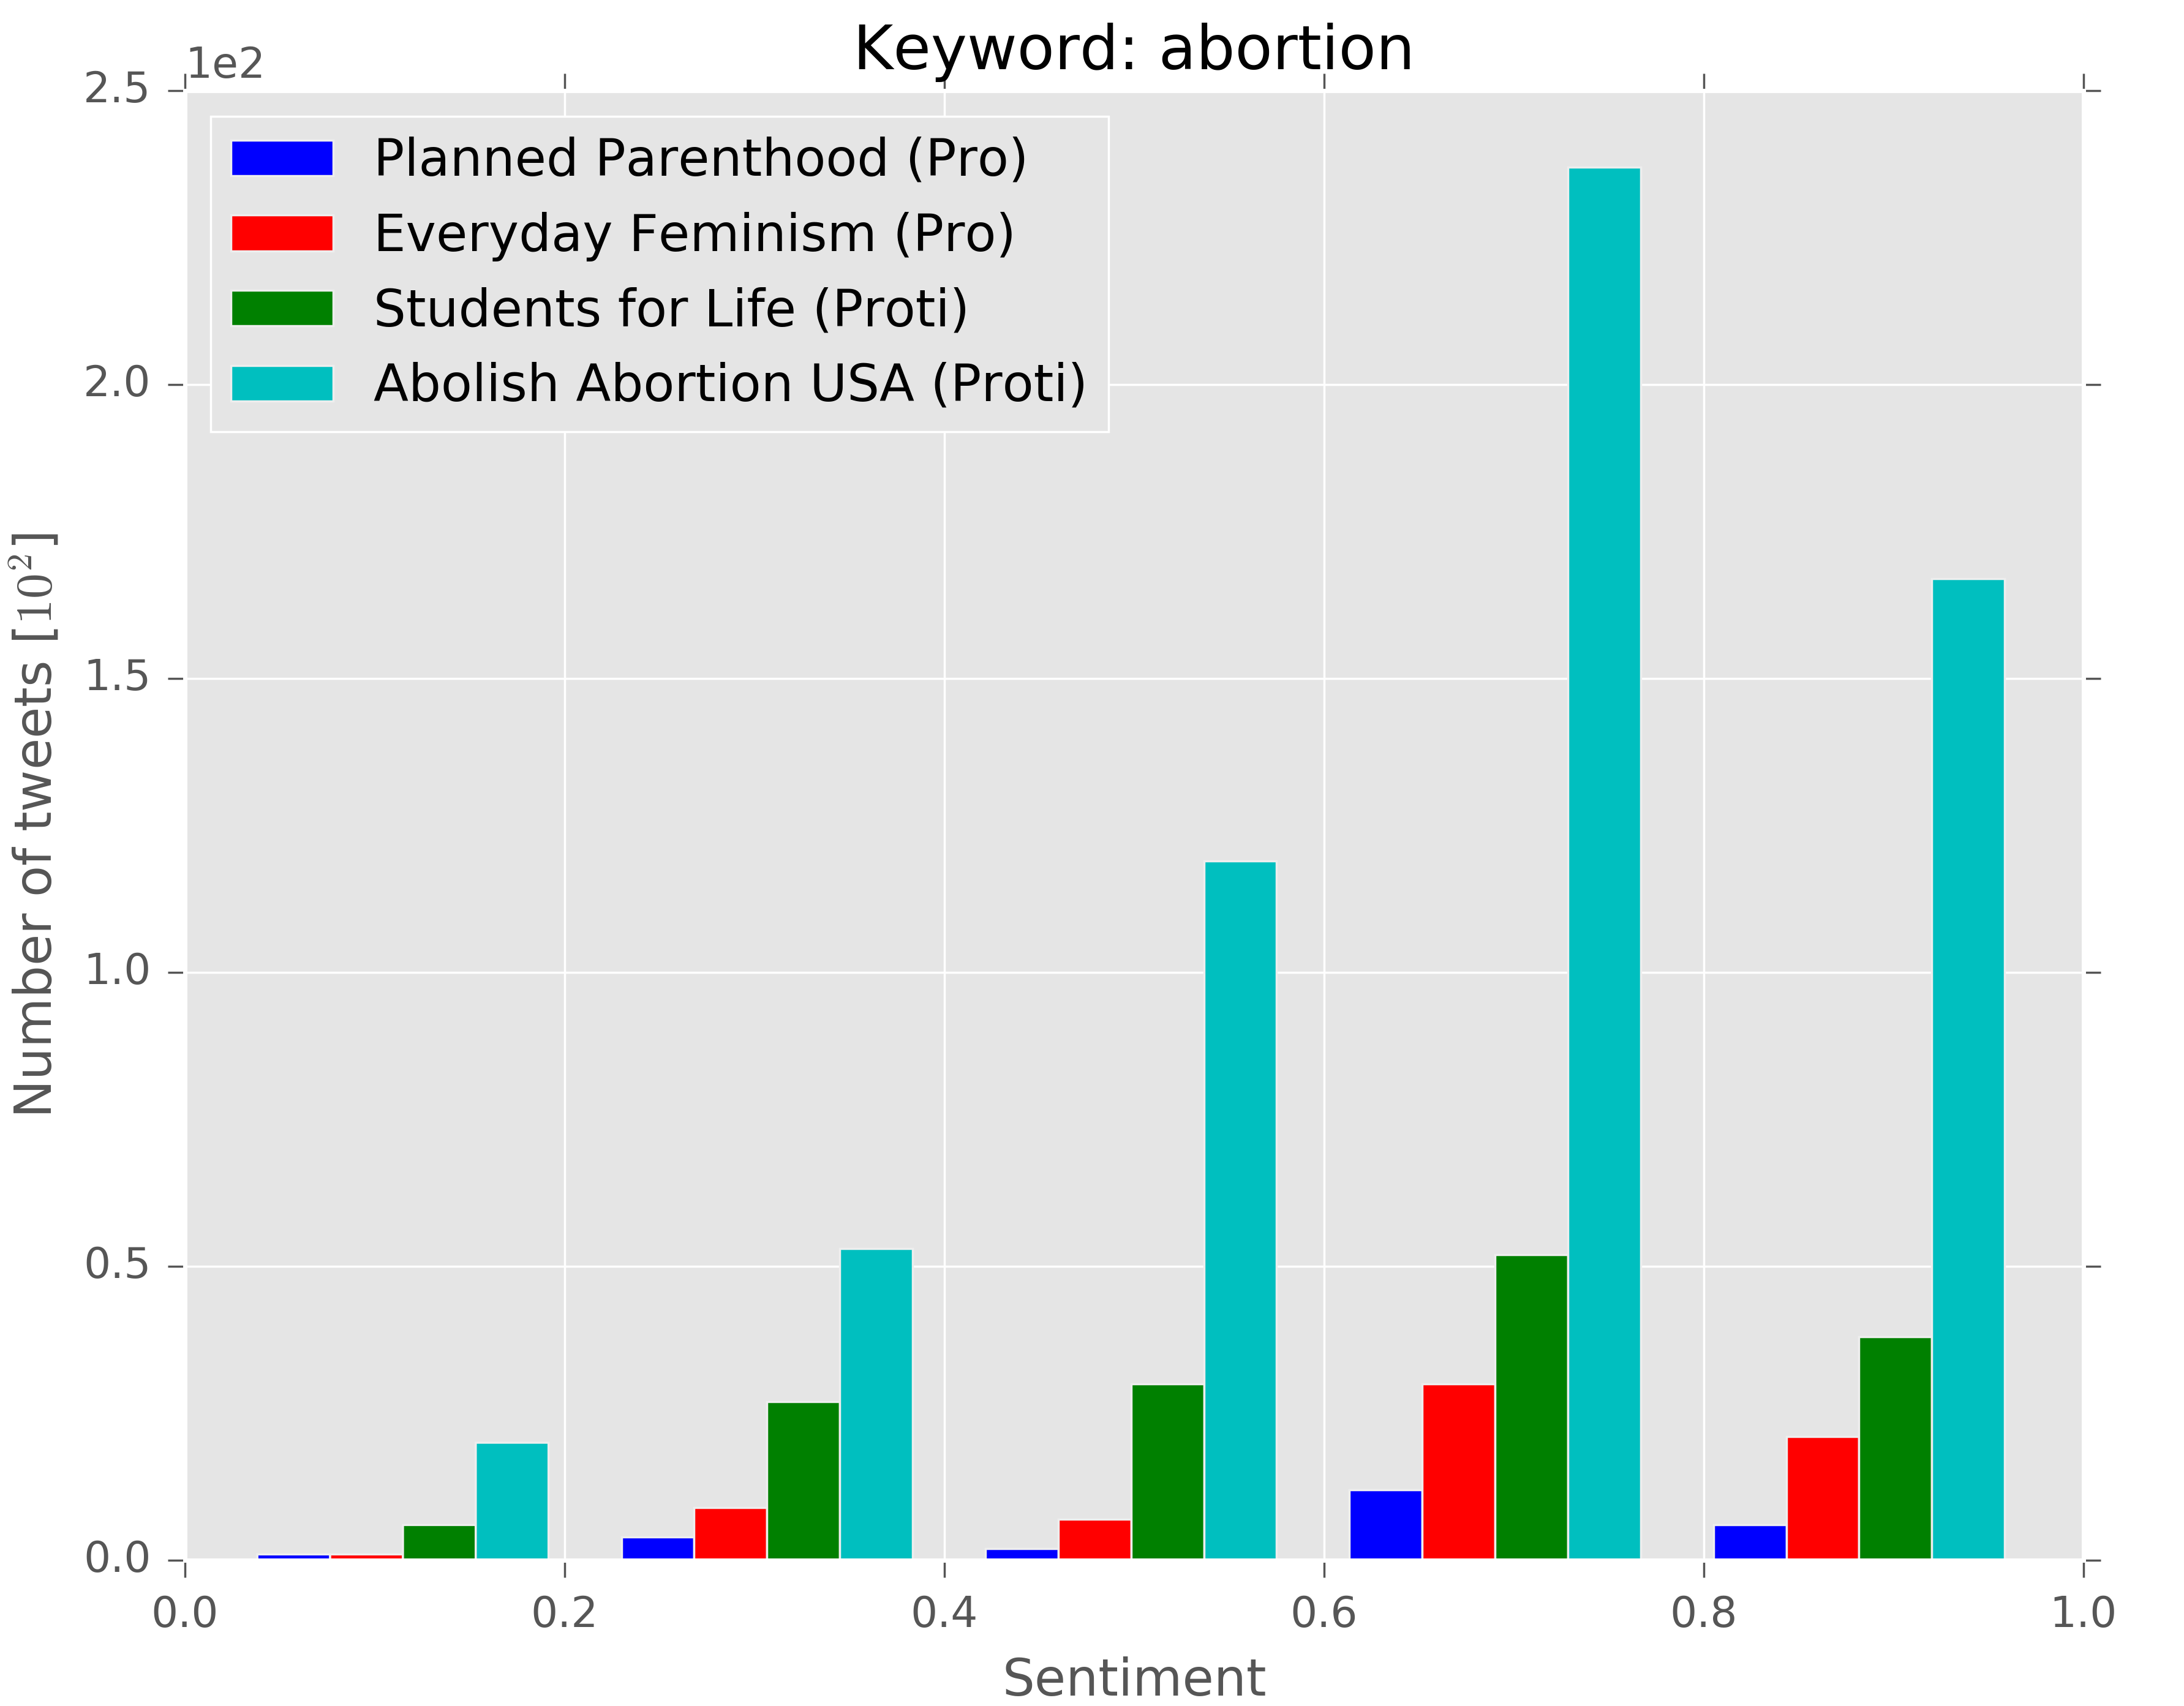
\includegraphics[scale=0.37]{./Pics/abortion.png}
    \end{figure}
    \vspace{-0.4cm}
    \begin{columns}
    \column{6cm}
    	\begin{itemize}
    		\item huge difference in number of tweets
            \item threat for objectivity
    	\end{itemize}
    \column{6cm}
    	\begin{itemize}
    		\item \textbf{more activity} in groups against abortion
        \end{itemize}
    \end{columns}
\end{frame}
% ############################################
\begin{frame}{Keyword: abortion}
    \begin{figure}
        \centering
        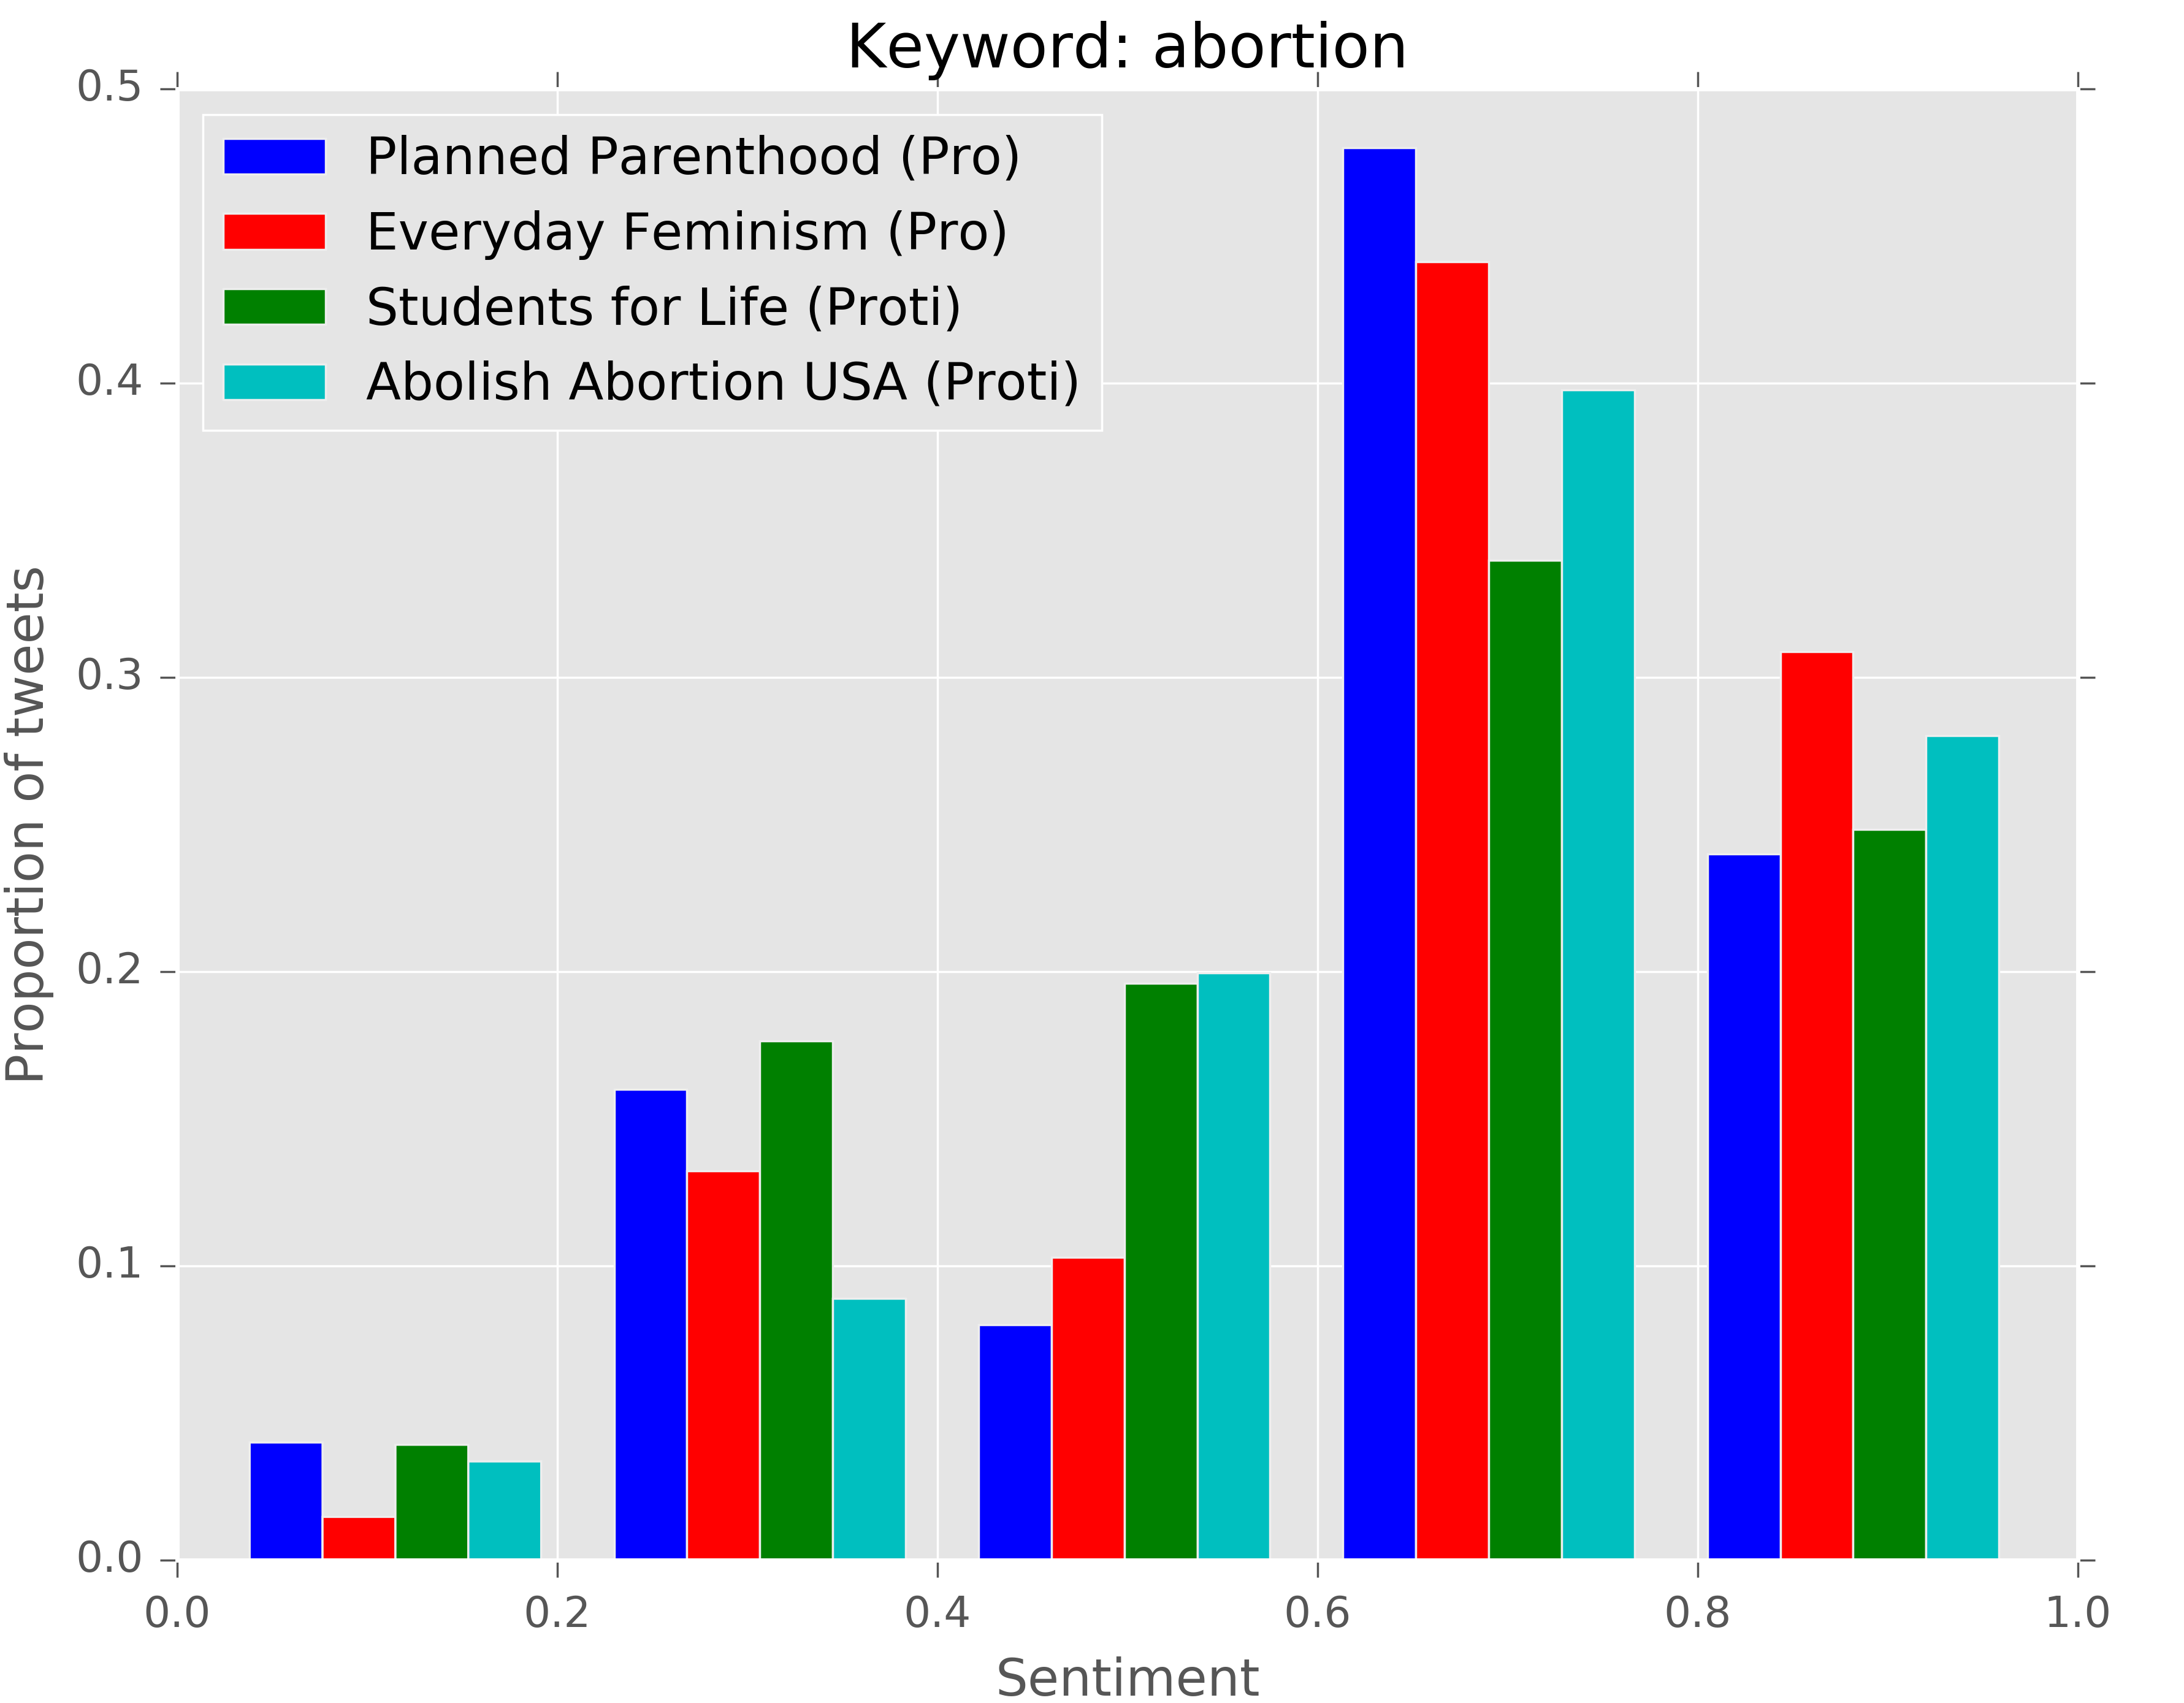
\includegraphics[scale=0.37]{./Pics/abortion-normed.png}
        \vspace{-0.2cm}
        \caption*{Normalized histogram - sentiment proportion.}
    \end{figure}
    \vspace{-0.4cm}
	\begin{itemize}
		\item against abortion $\rightarrow$ sentiment $< 0.5$
        \item for abortion $\rightarrow$ sentiment $> 0.5$
	\end{itemize}
\end{frame}
% ############################################
% ############################################
\begin{frame}{Conclusion}
    \begin{block}{New method:}
        \begin{itemize}
            \item large scale - \textbf{noise reduction}
            \item more \textbf{straightforward} than traditional research
            \item quantitative research
        \end{itemize}
    \end{block}

    \begin{block}{Measurements:}
    	\begin{itemize}
            \item Trump $\rightarrow$ low content homogenity
            \item abortion $\rightarrow$ \textbf{threat} for objectivity
    	\end{itemize}
    \end{block}
\end{frame}
% ############################################
% ############################################
\begin{frame}

\end{frame}
% ############################################
% ############################################
\begin{frame}{Tweet examples}
    \begin{block}{Everyday Feminism:}
        \begin{itemize}
            \item \begin{footnotesize} "\textit{We're proud of all of the abortion providers in this room - thank you for your brave; compassionate care. \#Proud2Provide \#LifesWork}" \end{footnotesize} (0.9776)
        \end{itemize}
    \end{block}
    \begin{block}{Abolish Abortion USA:}
        \begin{itemize}
            \item \begin{footnotesize} "\textit{And look at the Planned parenthood abortion rooms.....887 babies killed a day and 300,000 dead babies a year....!!!}" \end{footnotesize} (0.2255)
        \end{itemize}
    \end{block}
\end{frame}
\end{document}
